\documentclass[twoside]{book}

% Packages required by doxygen
\usepackage{fixltx2e}
\usepackage{calc}
\usepackage{doxygen}
\usepackage[export]{adjustbox} % also loads graphicx
\usepackage{graphicx}
\usepackage[utf8]{inputenc}
\usepackage{makeidx}
\usepackage{multicol}
\usepackage{multirow}
\PassOptionsToPackage{warn}{textcomp}
\usepackage{textcomp}
\usepackage[nointegrals]{wasysym}
\usepackage[table]{xcolor}

% Font selection
\usepackage[T1]{fontenc}
\usepackage[scaled=.90]{helvet}
\usepackage{courier}
\usepackage{amssymb}
\usepackage{sectsty}
\renewcommand{\familydefault}{\sfdefault}
\allsectionsfont{%
  \fontseries{bc}\selectfont%
  \color{darkgray}%
}
\renewcommand{\DoxyLabelFont}{%
  \fontseries{bc}\selectfont%
  \color{darkgray}%
}
\newcommand{\+}{\discretionary{\mbox{\scriptsize$\hookleftarrow$}}{}{}}

% Page & text layout
\usepackage{geometry}
\geometry{%
  a4paper,%
  top=2.5cm,%
  bottom=2.5cm,%
  left=2.5cm,%
  right=2.5cm%
}
\tolerance=750
\hfuzz=15pt
\hbadness=750
\setlength{\emergencystretch}{15pt}
\setlength{\parindent}{0cm}
\setlength{\parskip}{3ex plus 2ex minus 2ex}
\makeatletter
\renewcommand{\paragraph}{%
  \@startsection{paragraph}{4}{0ex}{-1.0ex}{1.0ex}{%
    \normalfont\normalsize\bfseries\SS@parafont%
  }%
}
\renewcommand{\subparagraph}{%
  \@startsection{subparagraph}{5}{0ex}{-1.0ex}{1.0ex}{%
    \normalfont\normalsize\bfseries\SS@subparafont%
  }%
}
\makeatother

% Headers & footers
\usepackage{fancyhdr}
\pagestyle{fancyplain}
\fancyhead[LE]{\fancyplain{}{\bfseries\thepage}}
\fancyhead[CE]{\fancyplain{}{}}
\fancyhead[RE]{\fancyplain{}{\bfseries\leftmark}}
\fancyhead[LO]{\fancyplain{}{\bfseries\rightmark}}
\fancyhead[CO]{\fancyplain{}{}}
\fancyhead[RO]{\fancyplain{}{\bfseries\thepage}}
\fancyfoot[LE]{\fancyplain{}{}}
\fancyfoot[CE]{\fancyplain{}{}}
\fancyfoot[RE]{\fancyplain{}{\bfseries\scriptsize Generated by Doxygen }}
\fancyfoot[LO]{\fancyplain{}{\bfseries\scriptsize Generated by Doxygen }}
\fancyfoot[CO]{\fancyplain{}{}}
\fancyfoot[RO]{\fancyplain{}{}}
\renewcommand{\footrulewidth}{0.4pt}
\renewcommand{\chaptermark}[1]{%
  \markboth{#1}{}%
}
\renewcommand{\sectionmark}[1]{%
  \markright{\thesection\ #1}%
}

% Indices & bibliography
\usepackage{natbib}
\usepackage[titles]{tocloft}
\setcounter{tocdepth}{3}
\setcounter{secnumdepth}{5}
\makeindex

% Hyperlinks (required, but should be loaded last)
\usepackage{ifpdf}
\ifpdf
  \usepackage[pdftex,pagebackref=true]{hyperref}
\else
  \usepackage[ps2pdf,pagebackref=true]{hyperref}
\fi
\hypersetup{%
  colorlinks=true,%
  linkcolor=blue,%
  citecolor=blue,%
  unicode%
}

% Custom commands
\newcommand{\clearemptydoublepage}{%
  \newpage{\pagestyle{empty}\cleardoublepage}%
}

\usepackage{caption}
\captionsetup{labelsep=space,justification=centering,font={bf},singlelinecheck=off,skip=4pt,position=top}

%===== C O N T E N T S =====

\begin{document}

% Titlepage & ToC
\hypersetup{pageanchor=false,
             bookmarksnumbered=true,
             pdfencoding=unicode
            }
\pagenumbering{alph}
\begin{titlepage}
\vspace*{7cm}
\begin{center}%
{\Large Marvinette }\\
\vspace*{1cm}
{\large Generated by Doxygen 1.8.13}\\
\end{center}
\end{titlepage}
\clearemptydoublepage
\pagenumbering{roman}
\tableofcontents
\clearemptydoublepage
\pagenumbering{arabic}
\hypersetup{pageanchor=true}

%--- Begin generated contents ---
\chapter{Main Page}
\label{index}\hypertarget{index}{}\href{images/logo.PNG}{\tt }

\href{https://github.com/Arthi-chaud/Marvinette/actions/workflows/unit_tests.yml}{\tt } \href{https://sonarcloud.io/dashboard?id=Arthi-chaud_Marvinette}{\tt } \href{https://sonarcloud.io/dashboard?id=Arthi-chaud_Marvinette}{\tt } \href{https://arthi-chaud.github.io/Marvinette/}{\tt } 




\begin{DoxyEnumerate}
\item Clone the repository
\item Move it to your {\ttfamily \$\+H\+O\+ME} folder (or a directory where you wouldn\textquotesingle{}t want to move the repository)
\item Inside the repository, execute the following command\+:
\end{DoxyEnumerate}


\begin{DoxyCode}
php MarvinetteInstall.php
\end{DoxyCode}


{\bfseries Warning} If installation fails, try installation using {\ttfamily sudo}


\begin{DoxyEnumerate}
\item (Only For Windows) Add the path of the marvinette folder to your {\ttfamily P\+A\+TH} environment variable
\end{DoxyEnumerate}

{\bfseries Warning}\+: Once you executed the command, you must not move the Marvinette folder. If you do, you\textquotesingle{}ll have to execute the install command again 




\begin{DoxyEnumerate}
\item Before anything else, you must create your project\textquotesingle{}s configuration file for Marvinette. To do so\+:
\begin{DoxyItemize}
\item go to your project\textquotesingle{}s directory
\item execute the following command\+:
\end{DoxyItemize}
\end{DoxyEnumerate}


\begin{DoxyCode}
marvinette --create-project
\end{DoxyCode}



\begin{DoxyItemize}
\item You will be prompt to enter several values.
\item You can modify your configuration file using the following command (avoid changing the file yourself)\+:
\end{DoxyItemize}


\begin{DoxyCode}
marvinette --mod-project
\end{DoxyCode}



\begin{DoxyEnumerate}
\item You can now create your first functional test!
\begin{DoxyItemize}
\item execute the command\+:
\end{DoxyItemize}
\end{DoxyEnumerate}


\begin{DoxyCode}
marvinette --add-test
\end{DoxyCode}



\begin{DoxyItemize}
\item You will be prompt to enter different values.
\item In your test\textquotesingle{}s folder, some files will be empty\+: you\textquotesingle{}ll have to fill them yourself (expected\+Stdout/\+Stderr, standard input, stdout/stderr\+Filter). If a file is empty, for example expected\+Stdout, the standard output of the program will be compared with the file\textquotesingle{}s content. If you don\textquotesingle{}t want to, simply delete the file.
\end{DoxyItemize}

Your tests are ready to be executed!
\begin{DoxyItemize}
\item To execute one test, execute the command\+:
\end{DoxyItemize}


\begin{DoxyCode}
marvinette --execute-test
\end{DoxyCode}


You will be asked to choose which test to execute
\begin{DoxyItemize}
\item To execute all your tests, execute the command\+:
\end{DoxyItemize}


\begin{DoxyCode}
marvinette --execute-tests
\end{DoxyCode}
 



Use the framework using the following command-\/line instructions\+:


\begin{DoxyCode}
marvinette [option]

  option:
    --create-project: Create a main configuration file, required to make tests
    --create-sample-project: Create a sample configuration file. The values will be changed by the user.
    --del-project, --delete-project: Delete configuration file and existing tests
    --mod-project: Modify the project\(\backslash\)'s info.

    --add-test, --create-test: Create a functional test
    --create-sample-test: Create a sample test file. The values will be changed by the user.
    --mod-test: Modify a functional test
    --del-test, --delete-test: Delete a functional test

    --execute-test,--exec-test : Execute a test
    --execute-tests, --exec-all  : Execute all tests

    -h, --help: display this usage
\end{DoxyCode}
 



The framework\textquotesingle{}s configuration file, {\ttfamily Marvinette.\+json}, holds the following information\+:


\begin{DoxyItemize}
\item {\ttfamily name}\+: The name of the project
\item {\ttfamily binary name}\+: the name of the binary/script to execute
\item {\ttfamily binary path}\+: the path to the binary/script
\item {\ttfamily interpreter}\+: the interpreter of the script (for example\+: python3 for a python script, or nothing for binary executables)
\item {\ttfamily tests folder}\+: the path to the tests\textquotesingle{} folder
\end{DoxyItemize}

If you do not want to use the command-\/line interface to configure your project, use the {\ttfamily -\/-\/create-\/sample-\/project}. It will create a sample configuration file and you change the values by yourself

Upon test creation, several files are generated in the {\ttfamily test\+Folder}/{\ttfamily test\+Name} folder\+:


\begin{DoxyItemize}
\item A {\ttfamily config.\+json} file, holding the following values\+:
\begin{DoxyItemize}
\item {\ttfamily command\+Line\+Arguments}\+: holds the arguments which will be passed to the program.
\item {\ttfamily interpreter\+Arguments}\+: holds the arguments which will be passed to the program\textquotesingle{}s interpreter. The arguments will be read only if an interpreter is set in the {\ttfamily Marvinette.\+json} file.
\item {\ttfamily expected\+Return\+Code}\+: the returned code expected from the program\textquotesingle{}s execution (if the field\textquotesingle{}s value is not a number, the comparison will be scrapped).
\item {\ttfamily stdout\+Filter}\+: the standard output the command will be piped onto.
\item {\ttfamily stderr\+Filter}\+: the error output the command will be piped onto.
\item {\ttfamily empty\+Env}\+: if true, the test command will be executed within an empty environment.
\item {\ttfamily setup}\+: this command will be executed before the program is launched.
\item {\ttfamily teardown}\+: this command will be executed after the program is launched.
\end{DoxyItemize}
\end{DoxyItemize}

Any of the fields can be null. If that\textquotesingle{}s the case, the described action will not be executed.


\begin{DoxyItemize}
\item {\ttfamily stdinput}\+: if the file exists, the content of the file will be standard input to the program.
\item {\ttfamily expected\+Stdout}\+: if the file exists, the (filtered) standard output will be compared to the file\textquotesingle{}s content. If there is no such file, no comparison will be done.
\item {\ttfamily expected\+Stderr}\+: if the file exists, the (filtered) error output will be compared to the file\textquotesingle{}s content. If there is no such file, no comparison will be done.
\end{DoxyItemize}

If a {\ttfamily setup}, {\ttfamily stdout/stderr\+Filter} or {\ttfamily teardown} command doesn\textquotesingle{}t return 0, the test will fail.

Upon creation, feel free to change the files\textquotesingle{} content by yourself. Be careful not to leave any {\itshape useless} line breaks of trailing spaces 



You can use Marvinette on an Unix-\/based OS or on Windows!

Also, you\textquotesingle{}ll need P\+HP $>$= 7.\+4. No other library needed (the {\ttfamily vendor} folder and composer configuration file are used for Marvinette\textquotesingle{}s unit tests) 



\href{https://sonarcloud.io/dashboard?id=Arthi-chaud_Marvinette}{\tt } 
\chapter{Hierarchical Index}
\section{Class Hierarchy}
This inheritance list is sorted roughly, but not completely, alphabetically\+:\begin{DoxyCompactList}
\item \contentsline{section}{Display\textbackslash{}Color}{\pageref{classDisplay_1_1Color}}{}
\item \contentsline{section}{Display\textbackslash{}Displayer}{\pageref{classDisplay_1_1Displayer}}{}
\item Exception\begin{DoxyCompactList}
\item \contentsline{section}{Marvinette\+Exception}{\pageref{classMarvinetteException}}{}
\begin{DoxyCompactList}
\item \contentsline{section}{End\+Of\+File\+Exception}{\pageref{classEndOfFileException}}{}
\item \contentsline{section}{Invalid\+Config\+File\+Exception}{\pageref{classInvalidConfigFileException}}{}
\item \contentsline{section}{Invalid\+Test\+Folder\+Exception}{\pageref{classInvalidTestFolderException}}{}
\item \contentsline{section}{No\+Config\+File\+Exception}{\pageref{classNoConfigFileException}}{}
\end{DoxyCompactList}
\end{DoxyCompactList}
\item \contentsline{section}{Field}{\pageref{classField}}{}
\item \contentsline{section}{File\+Manager}{\pageref{classFileManager}}{}
\item \contentsline{section}{Object\+Helper}{\pageref{classObjectHelper}}{}
\item \contentsline{section}{Project}{\pageref{classProject}}{}
\item \contentsline{section}{Project\+Manager}{\pageref{classProjectManager}}{}
\item \contentsline{section}{Display\textbackslash{}Style}{\pageref{classDisplay_1_1Style}}{}
\item \contentsline{section}{Test}{\pageref{classTest}}{}
\item \contentsline{section}{Test\+Manager}{\pageref{classTestManager}}{}
\item \contentsline{section}{User\+Input}{\pageref{classUserInput}}{}
\item \contentsline{section}{User\+Interface}{\pageref{classUserInterface}}{}
\end{DoxyCompactList}

\chapter{Class Index}
\section{Class List}
Here are the classes, structs, unions and interfaces with brief descriptions\+:\begin{DoxyCompactList}
\item\contentsline{section}{\hyperlink{classDisplay_1_1Color}{Display\textbackslash{}\+Color} \\*Static class holding color int for terminal display }{\pageref{classDisplay_1_1Color}}{}
\item\contentsline{section}{\hyperlink{classDisplay_1_1Displayer}{Display\textbackslash{}\+Displayer} \\*Display utility class }{\pageref{classDisplay_1_1Displayer}}{}
\item\contentsline{section}{\hyperlink{classEndOfFileException}{End\+Of\+File\+Exception} }{\pageref{classEndOfFileException}}{}
\item\contentsline{section}{\hyperlink{classField}{Field} \\*Object representing a class\textquotesingle{}s variable member, but allows error handling and prompt help messages }{\pageref{classField}}{}
\item\contentsline{section}{\hyperlink{classFileManager}{File\+Manager} }{\pageref{classFileManager}}{}
\item\contentsline{section}{\hyperlink{classInvalidConfigFileException}{Invalid\+Config\+File\+Exception} }{\pageref{classInvalidConfigFileException}}{}
\item\contentsline{section}{\hyperlink{classInvalidTestFolderException}{Invalid\+Test\+Folder\+Exception} }{\pageref{classInvalidTestFolderException}}{}
\item\contentsline{section}{\hyperlink{classMarvinetteException}{Marvinette\+Exception} }{\pageref{classMarvinetteException}}{}
\item\contentsline{section}{\hyperlink{classNoConfigFileException}{No\+Config\+File\+Exception} }{\pageref{classNoConfigFileException}}{}
\item\contentsline{section}{\hyperlink{classObjectHelper}{Object\+Helper} }{\pageref{classObjectHelper}}{}
\item\contentsline{section}{\hyperlink{classProject}{Project} \\*Object representing the project\textquotesingle{}s important infos }{\pageref{classProject}}{}
\item\contentsline{section}{\hyperlink{classProjectManager}{Project\+Manager} }{\pageref{classProjectManager}}{}
\item\contentsline{section}{\hyperlink{classDisplay_1_1Style}{Display\textbackslash{}\+Style} \\*Static class holding style int for terminal display }{\pageref{classDisplay_1_1Style}}{}
\item\contentsline{section}{\hyperlink{classTest}{Test} \\*Object representing the test\textquotesingle{}s instruction }{\pageref{classTest}}{}
\item\contentsline{section}{\hyperlink{classTestManager}{Test\+Manager} }{\pageref{classTestManager}}{}
\item\contentsline{section}{\hyperlink{classUserInput}{User\+Input} }{\pageref{classUserInput}}{}
\item\contentsline{section}{\hyperlink{classUserInterface}{User\+Interface} \\*Everythong related to user interface }{\pageref{classUserInterface}}{}
\end{DoxyCompactList}

\chapter{Class Documentation}
\hypertarget{classDisplay_1_1Color}{}\section{Display\textbackslash{}Color Class Reference}
\label{classDisplay_1_1Color}\index{Display\textbackslash{}\+Color@{Display\textbackslash{}\+Color}}


static class holding color int for terminal display  


\subsection*{Public Attributes}
\begin{DoxyCompactItemize}
\item 
\mbox{\Hypertarget{classDisplay_1_1Color_aeaa09b4902c94778eda993ae01af2dfb}\label{classDisplay_1_1Color_aeaa09b4902c94778eda993ae01af2dfb}} 
const \hyperlink{classDisplay_1_1Color_aeaa09b4902c94778eda993ae01af2dfb}{B\+A\+C\+K\+G\+R\+O\+U\+N\+D\+\_\+\+O\+F\+F\+S\+ET} = 10
\begin{DoxyCompactList}\small\item\em Offsert between text color and backgorund color (used for avoid creating another class) \end{DoxyCompactList}\item 
\mbox{\Hypertarget{classDisplay_1_1Color_a667403f6acc19e11a5edeae75ca44c6d}\label{classDisplay_1_1Color_a667403f6acc19e11a5edeae75ca44c6d}} 
const \hyperlink{classDisplay_1_1Color_a667403f6acc19e11a5edeae75ca44c6d}{Default} = 39
\begin{DoxyCompactList}\small\item\em id letting the terminal know to write using the default color \end{DoxyCompactList}\item 
\mbox{\Hypertarget{classDisplay_1_1Color_afc2c98adc048bfe0d7c627239781ca10}\label{classDisplay_1_1Color_afc2c98adc048bfe0d7c627239781ca10}} 
const \hyperlink{classDisplay_1_1Color_afc2c98adc048bfe0d7c627239781ca10}{Black} = 30
\begin{DoxyCompactList}\small\item\em id letting the terminal know to write using black \end{DoxyCompactList}\item 
\mbox{\Hypertarget{classDisplay_1_1Color_a6b0b1dff4e3cfd9f0b7fb118c8c23e9b}\label{classDisplay_1_1Color_a6b0b1dff4e3cfd9f0b7fb118c8c23e9b}} 
const \hyperlink{classDisplay_1_1Color_a6b0b1dff4e3cfd9f0b7fb118c8c23e9b}{Red} = 31
\begin{DoxyCompactList}\small\item\em id letting the terminal know to write using red \end{DoxyCompactList}\item 
\mbox{\Hypertarget{classDisplay_1_1Color_aeb788f34802227529b2f711246677052}\label{classDisplay_1_1Color_aeb788f34802227529b2f711246677052}} 
const \hyperlink{classDisplay_1_1Color_aeb788f34802227529b2f711246677052}{Green} = 32
\begin{DoxyCompactList}\small\item\em id letting the terminal know to write using green \end{DoxyCompactList}\item 
\mbox{\Hypertarget{classDisplay_1_1Color_ade208f3dbf1e9713dbc07a3f8e45377c}\label{classDisplay_1_1Color_ade208f3dbf1e9713dbc07a3f8e45377c}} 
const \hyperlink{classDisplay_1_1Color_ade208f3dbf1e9713dbc07a3f8e45377c}{Yellow} = 33
\begin{DoxyCompactList}\small\item\em id letting the terminal know to write using yellow \end{DoxyCompactList}\item 
\mbox{\Hypertarget{classDisplay_1_1Color_ac8a29dad37837402d832bc0fae4d7096}\label{classDisplay_1_1Color_ac8a29dad37837402d832bc0fae4d7096}} 
const \hyperlink{classDisplay_1_1Color_ac8a29dad37837402d832bc0fae4d7096}{Blue} = 34
\begin{DoxyCompactList}\small\item\em id letting the terminal know to write using blue \end{DoxyCompactList}\item 
\mbox{\Hypertarget{classDisplay_1_1Color_aa3899d6446d5ccfa3cd1ac41a91596bc}\label{classDisplay_1_1Color_aa3899d6446d5ccfa3cd1ac41a91596bc}} 
const \hyperlink{classDisplay_1_1Color_aa3899d6446d5ccfa3cd1ac41a91596bc}{Magenta} = 35
\begin{DoxyCompactList}\small\item\em id letting the terminal know to write using magenta \end{DoxyCompactList}\item 
\mbox{\Hypertarget{classDisplay_1_1Color_a1a7382499f34f1c74a2b66459e481ac8}\label{classDisplay_1_1Color_a1a7382499f34f1c74a2b66459e481ac8}} 
const \hyperlink{classDisplay_1_1Color_a1a7382499f34f1c74a2b66459e481ac8}{Cyan} = 36
\begin{DoxyCompactList}\small\item\em id letting the terminal know to write using cyan \end{DoxyCompactList}\item 
\mbox{\Hypertarget{classDisplay_1_1Color_aec8bd907ba4fced890461a63c4cd4636}\label{classDisplay_1_1Color_aec8bd907ba4fced890461a63c4cd4636}} 
const \hyperlink{classDisplay_1_1Color_aec8bd907ba4fced890461a63c4cd4636}{Light\+Gray} = 37
\begin{DoxyCompactList}\small\item\em id letting the terminal know to write using light gray \end{DoxyCompactList}\item 
\mbox{\Hypertarget{classDisplay_1_1Color_a2c7f9964a522e822b13cc9321fdb9869}\label{classDisplay_1_1Color_a2c7f9964a522e822b13cc9321fdb9869}} 
const \hyperlink{classDisplay_1_1Color_a2c7f9964a522e822b13cc9321fdb9869}{Dark\+Gray} = 90
\begin{DoxyCompactList}\small\item\em id letting the terminal know to write using dark gray \end{DoxyCompactList}\item 
\mbox{\Hypertarget{classDisplay_1_1Color_a6e33fcb0f0da015e2d7c1bf2e9994341}\label{classDisplay_1_1Color_a6e33fcb0f0da015e2d7c1bf2e9994341}} 
const \hyperlink{classDisplay_1_1Color_a6e33fcb0f0da015e2d7c1bf2e9994341}{Light\+Red} = 91
\begin{DoxyCompactList}\small\item\em id letting the terminal know to write using light red \end{DoxyCompactList}\item 
\mbox{\Hypertarget{classDisplay_1_1Color_af745d885e59a992b69ed0155e25375a4}\label{classDisplay_1_1Color_af745d885e59a992b69ed0155e25375a4}} 
const \hyperlink{classDisplay_1_1Color_af745d885e59a992b69ed0155e25375a4}{Light\+Green} = 92
\begin{DoxyCompactList}\small\item\em id letting the terminal know to write using light green \end{DoxyCompactList}\item 
\mbox{\Hypertarget{classDisplay_1_1Color_acbc4c132efc5fc18eabc91be7750124f}\label{classDisplay_1_1Color_acbc4c132efc5fc18eabc91be7750124f}} 
const \hyperlink{classDisplay_1_1Color_acbc4c132efc5fc18eabc91be7750124f}{Light\+Yellow} = 93
\begin{DoxyCompactList}\small\item\em id letting the terminal know to write using light yellow \end{DoxyCompactList}\item 
\mbox{\Hypertarget{classDisplay_1_1Color_a2e01836e6c626de1fba9da114c6ec727}\label{classDisplay_1_1Color_a2e01836e6c626de1fba9da114c6ec727}} 
const \hyperlink{classDisplay_1_1Color_a2e01836e6c626de1fba9da114c6ec727}{Light\+Blue} = 94
\begin{DoxyCompactList}\small\item\em id letting the terminal know to write using light blue \end{DoxyCompactList}\item 
\mbox{\Hypertarget{classDisplay_1_1Color_a3ac22ad612cbcc41c0a67708b920bbe8}\label{classDisplay_1_1Color_a3ac22ad612cbcc41c0a67708b920bbe8}} 
const \hyperlink{classDisplay_1_1Color_a3ac22ad612cbcc41c0a67708b920bbe8}{Light\+Magenta} = 95
\begin{DoxyCompactList}\small\item\em id letting the terminal know to write using light magenta \end{DoxyCompactList}\item 
\mbox{\Hypertarget{classDisplay_1_1Color_a7e5ed177ee2f35031535e56281660ac4}\label{classDisplay_1_1Color_a7e5ed177ee2f35031535e56281660ac4}} 
const \hyperlink{classDisplay_1_1Color_a7e5ed177ee2f35031535e56281660ac4}{Light\+Cyan} = 96
\begin{DoxyCompactList}\small\item\em id letting the terminal know to write using light cyan \end{DoxyCompactList}\item 
\mbox{\Hypertarget{classDisplay_1_1Color_aa1e0bc8eacc7a1430e5e408f8f569bbb}\label{classDisplay_1_1Color_aa1e0bc8eacc7a1430e5e408f8f569bbb}} 
const \hyperlink{classDisplay_1_1Color_aa1e0bc8eacc7a1430e5e408f8f569bbb}{White} = 97
\begin{DoxyCompactList}\small\item\em id letting the terminal know to write using white \end{DoxyCompactList}\end{DoxyCompactItemize}


\subsection{Detailed Description}
static class holding color int for terminal display 

The documentation for this class was generated from the following file\+:\begin{DoxyCompactItemize}
\item 
src/\+Display/Color.\+php\end{DoxyCompactItemize}

\hypertarget{classDisplay_1_1Displayer}{}\section{Display\textbackslash{}Displayer Class Reference}
\label{classDisplay_1_1Displayer}\index{Display\textbackslash{}\+Displayer@{Display\textbackslash{}\+Displayer}}


Display utility class.  


\subsection*{Public Member Functions}
\begin{DoxyCompactItemize}
\item 
\hyperlink{classDisplay_1_1Displayer_a2e7ce80672e8e2433dce68eb7850090d}{display\+Text} (string \$text, bool \$newline=true, bool \$reset\+After=true)
\item 
\hyperlink{classDisplay_1_1Displayer_ac1a45d0e8bfd18db8a841172df12b44d}{get\+Color} ()
\item 
\hyperlink{classDisplay_1_1Displayer_a2df23fef055ca84673a9a90f55f3e3ee}{set\+Color} (\$color)
\item 
\hyperlink{classDisplay_1_1Displayer_af1da840727c16ebc4f08bbec07e5f86a}{reset\+Color} ()
\item 
\hyperlink{classDisplay_1_1Displayer_a3db965b4e13997094ba8527bfee8e60f}{get\+Background} ()
\item 
\hyperlink{classDisplay_1_1Displayer_ada8b108ad4678f8f94337748db34a062}{set\+Background} (\$background)
\item 
\hyperlink{classDisplay_1_1Displayer_afd285ad90f1eb4341a370f17ff7ab725}{reset\+Background} ()
\item 
\hyperlink{classDisplay_1_1Displayer_af1a84beba7ba2afd60dbe13814db5f42}{get\+Styles} ()
\item 
\hyperlink{classDisplay_1_1Displayer_ab9ba6574d40f5ecd249e461ac7e376b5}{set\+Style} (\$style)
\item 
\hyperlink{classDisplay_1_1Displayer_a2f6f5f0314cdb53ea96baa7dda489154}{set\+Styles} (array \$styles)
\item 
\hyperlink{classDisplay_1_1Displayer_ad30a8f26128fb57aa7b862a7eb899c0b}{reset\+Styles} ()
\item 
\hyperlink{classDisplay_1_1Displayer_a99a0bbaef46d045ad055692abaf153c3}{set} (array \$styles, \$color, \$background)
\item 
\hyperlink{classDisplay_1_1Displayer_a42bb7920ed6bc44c6e08747b87b1de63}{reset\+All} ()
\end{DoxyCompactItemize}
\subsection*{Protected Member Functions}
\begin{DoxyCompactItemize}
\item 
\hyperlink{classDisplay_1_1Displayer_a51f8584319905e94fd622a91a79072f8}{get\+Sequence} (\$id)
\end{DoxyCompactItemize}
\subsection*{Protected Attributes}
\begin{DoxyCompactItemize}
\item 
\mbox{\Hypertarget{classDisplay_1_1Displayer_a54d4898c73256f0c3b02616cf1bab7fd}\label{classDisplay_1_1Displayer_a54d4898c73256f0c3b02616cf1bab7fd}} 
{\bfseries \$color} = \hyperlink{classDisplay_1_1Color_a667403f6acc19e11a5edeae75ca44c6d}{Color\+::\+Default}
\item 
\mbox{\Hypertarget{classDisplay_1_1Displayer_aa3aa38460d82a6f85298eb84dd369513}\label{classDisplay_1_1Displayer_aa3aa38460d82a6f85298eb84dd369513}} 
array {\bfseries \$styles} = \mbox{[}$\,$\mbox{]}
\item 
\mbox{\Hypertarget{classDisplay_1_1Displayer_a254583ce5b771169dff389a30b82a54d}\label{classDisplay_1_1Displayer_a254583ce5b771169dff389a30b82a54d}} 
{\bfseries \$background} = \hyperlink{classDisplay_1_1Color_a667403f6acc19e11a5edeae75ca44c6d}{Color\+::\+Default}
\end{DoxyCompactItemize}


\subsection{Detailed Description}
Display utility class. 

\subsection{Member Function Documentation}
\mbox{\Hypertarget{classDisplay_1_1Displayer_a2e7ce80672e8e2433dce68eb7850090d}\label{classDisplay_1_1Displayer_a2e7ce80672e8e2433dce68eb7850090d}} 
\index{Display\+::\+Displayer@{Display\+::\+Displayer}!display\+Text@{display\+Text}}
\index{display\+Text@{display\+Text}!Display\+::\+Displayer@{Display\+::\+Displayer}}
\subsubsection{\texorpdfstring{display\+Text()}{displayText()}}
{\footnotesize\ttfamily Display\textbackslash{}\+Displayer\+::display\+Text (\begin{DoxyParamCaption}\item[{string}]{\$text,  }\item[{bool}]{\$newline = {\ttfamily true},  }\item[{bool}]{\$reset\+After = {\ttfamily true} }\end{DoxyParamCaption})}

Print text on S\+T\+D\+O\+UT, using set style / color / background. No format will be displayed if the S\+T\+D\+O\+UT is a T\+TY 
\begin{DoxyParams}[1]{Parameters}
string & {\em \$text} & the text to display \\
\hline
bool & {\em \$newline} & if true, a newline is displayed after the text \\
\hline
bool & {\em \$reset\+After} & if true, resets style / color / background \\
\hline
\end{DoxyParams}
\begin{DoxyReturn}{Returns}
self 
\end{DoxyReturn}
\mbox{\Hypertarget{classDisplay_1_1Displayer_a3db965b4e13997094ba8527bfee8e60f}\label{classDisplay_1_1Displayer_a3db965b4e13997094ba8527bfee8e60f}} 
\index{Display\+::\+Displayer@{Display\+::\+Displayer}!get\+Background@{get\+Background}}
\index{get\+Background@{get\+Background}!Display\+::\+Displayer@{Display\+::\+Displayer}}
\subsubsection{\texorpdfstring{get\+Background()}{getBackground()}}
{\footnotesize\ttfamily Display\textbackslash{}\+Displayer\+::get\+Background (\begin{DoxyParamCaption}{ }\end{DoxyParamCaption})}

Get the value of background \mbox{\Hypertarget{classDisplay_1_1Displayer_ac1a45d0e8bfd18db8a841172df12b44d}\label{classDisplay_1_1Displayer_ac1a45d0e8bfd18db8a841172df12b44d}} 
\index{Display\+::\+Displayer@{Display\+::\+Displayer}!get\+Color@{get\+Color}}
\index{get\+Color@{get\+Color}!Display\+::\+Displayer@{Display\+::\+Displayer}}
\subsubsection{\texorpdfstring{get\+Color()}{getColor()}}
{\footnotesize\ttfamily Display\textbackslash{}\+Displayer\+::get\+Color (\begin{DoxyParamCaption}{ }\end{DoxyParamCaption})}

Get the value of color \mbox{\Hypertarget{classDisplay_1_1Displayer_a51f8584319905e94fd622a91a79072f8}\label{classDisplay_1_1Displayer_a51f8584319905e94fd622a91a79072f8}} 
\index{Display\+::\+Displayer@{Display\+::\+Displayer}!get\+Sequence@{get\+Sequence}}
\index{get\+Sequence@{get\+Sequence}!Display\+::\+Displayer@{Display\+::\+Displayer}}
\subsubsection{\texorpdfstring{get\+Sequence()}{getSequence()}}
{\footnotesize\ttfamily Display\textbackslash{}\+Displayer\+::get\+Sequence (\begin{DoxyParamCaption}\item[{}]{\$id }\end{DoxyParamCaption})\hspace{0.3cm}{\ttfamily [protected]}}


\begin{DoxyParams}[1]{Parameters}
int & {\em \$id} & the ID of the style/color \\
\hline
\end{DoxyParams}
\begin{DoxyReturn}{Returns}
string formatted string for terminal setting 
\end{DoxyReturn}
\mbox{\Hypertarget{classDisplay_1_1Displayer_af1a84beba7ba2afd60dbe13814db5f42}\label{classDisplay_1_1Displayer_af1a84beba7ba2afd60dbe13814db5f42}} 
\index{Display\+::\+Displayer@{Display\+::\+Displayer}!get\+Styles@{get\+Styles}}
\index{get\+Styles@{get\+Styles}!Display\+::\+Displayer@{Display\+::\+Displayer}}
\subsubsection{\texorpdfstring{get\+Styles()}{getStyles()}}
{\footnotesize\ttfamily Display\textbackslash{}\+Displayer\+::get\+Styles (\begin{DoxyParamCaption}{ }\end{DoxyParamCaption})}

Get the value of style \mbox{\Hypertarget{classDisplay_1_1Displayer_a42bb7920ed6bc44c6e08747b87b1de63}\label{classDisplay_1_1Displayer_a42bb7920ed6bc44c6e08747b87b1de63}} 
\index{Display\+::\+Displayer@{Display\+::\+Displayer}!reset\+All@{reset\+All}}
\index{reset\+All@{reset\+All}!Display\+::\+Displayer@{Display\+::\+Displayer}}
\subsubsection{\texorpdfstring{reset\+All()}{resetAll()}}
{\footnotesize\ttfamily Display\textbackslash{}\+Displayer\+::reset\+All (\begin{DoxyParamCaption}{ }\end{DoxyParamCaption})}

resets all presets values, using rest memeber functions \mbox{\Hypertarget{classDisplay_1_1Displayer_afd285ad90f1eb4341a370f17ff7ab725}\label{classDisplay_1_1Displayer_afd285ad90f1eb4341a370f17ff7ab725}} 
\index{Display\+::\+Displayer@{Display\+::\+Displayer}!reset\+Background@{reset\+Background}}
\index{reset\+Background@{reset\+Background}!Display\+::\+Displayer@{Display\+::\+Displayer}}
\subsubsection{\texorpdfstring{reset\+Background()}{resetBackground()}}
{\footnotesize\ttfamily Display\textbackslash{}\+Displayer\+::reset\+Background (\begin{DoxyParamCaption}{ }\end{DoxyParamCaption})}

Reset Background color value to default \mbox{\Hypertarget{classDisplay_1_1Displayer_af1da840727c16ebc4f08bbec07e5f86a}\label{classDisplay_1_1Displayer_af1da840727c16ebc4f08bbec07e5f86a}} 
\index{Display\+::\+Displayer@{Display\+::\+Displayer}!reset\+Color@{reset\+Color}}
\index{reset\+Color@{reset\+Color}!Display\+::\+Displayer@{Display\+::\+Displayer}}
\subsubsection{\texorpdfstring{reset\+Color()}{resetColor()}}
{\footnotesize\ttfamily Display\textbackslash{}\+Displayer\+::reset\+Color (\begin{DoxyParamCaption}{ }\end{DoxyParamCaption})}

Set color field to null

\begin{DoxyReturn}{Returns}
self 
\end{DoxyReturn}
\mbox{\Hypertarget{classDisplay_1_1Displayer_ad30a8f26128fb57aa7b862a7eb899c0b}\label{classDisplay_1_1Displayer_ad30a8f26128fb57aa7b862a7eb899c0b}} 
\index{Display\+::\+Displayer@{Display\+::\+Displayer}!reset\+Styles@{reset\+Styles}}
\index{reset\+Styles@{reset\+Styles}!Display\+::\+Displayer@{Display\+::\+Displayer}}
\subsubsection{\texorpdfstring{reset\+Styles()}{resetStyles()}}
{\footnotesize\ttfamily Display\textbackslash{}\+Displayer\+::reset\+Styles (\begin{DoxyParamCaption}{ }\end{DoxyParamCaption})}

Reset Styles values, the array is emptied \mbox{\Hypertarget{classDisplay_1_1Displayer_a99a0bbaef46d045ad055692abaf153c3}\label{classDisplay_1_1Displayer_a99a0bbaef46d045ad055692abaf153c3}} 
\index{Display\+::\+Displayer@{Display\+::\+Displayer}!set@{set}}
\index{set@{set}!Display\+::\+Displayer@{Display\+::\+Displayer}}
\subsubsection{\texorpdfstring{set()}{set()}}
{\footnotesize\ttfamily Display\textbackslash{}\+Displayer\+::set (\begin{DoxyParamCaption}\item[{array}]{\$styles,  }\item[{}]{\$color,  }\item[{}]{\$background }\end{DoxyParamCaption})}

Set styles and color to use 
\begin{DoxyParams}{Parameters}
{\em Display} & \\
\hline
\end{DoxyParams}
\mbox{\Hypertarget{classDisplay_1_1Displayer_ada8b108ad4678f8f94337748db34a062}\label{classDisplay_1_1Displayer_ada8b108ad4678f8f94337748db34a062}} 
\index{Display\+::\+Displayer@{Display\+::\+Displayer}!set\+Background@{set\+Background}}
\index{set\+Background@{set\+Background}!Display\+::\+Displayer@{Display\+::\+Displayer}}
\subsubsection{\texorpdfstring{set\+Background()}{setBackground()}}
{\footnotesize\ttfamily Display\textbackslash{}\+Displayer\+::set\+Background (\begin{DoxyParamCaption}\item[{}]{\$background }\end{DoxyParamCaption})}

Set the value of background

\begin{DoxyReturn}{Returns}
self 
\end{DoxyReturn}
\mbox{\Hypertarget{classDisplay_1_1Displayer_a2df23fef055ca84673a9a90f55f3e3ee}\label{classDisplay_1_1Displayer_a2df23fef055ca84673a9a90f55f3e3ee}} 
\index{Display\+::\+Displayer@{Display\+::\+Displayer}!set\+Color@{set\+Color}}
\index{set\+Color@{set\+Color}!Display\+::\+Displayer@{Display\+::\+Displayer}}
\subsubsection{\texorpdfstring{set\+Color()}{setColor()}}
{\footnotesize\ttfamily Display\textbackslash{}\+Displayer\+::set\+Color (\begin{DoxyParamCaption}\item[{}]{\$color }\end{DoxyParamCaption})}

Set the value of color

\begin{DoxyReturn}{Returns}
self 
\end{DoxyReturn}
\mbox{\Hypertarget{classDisplay_1_1Displayer_ab9ba6574d40f5ecd249e461ac7e376b5}\label{classDisplay_1_1Displayer_ab9ba6574d40f5ecd249e461ac7e376b5}} 
\index{Display\+::\+Displayer@{Display\+::\+Displayer}!set\+Style@{set\+Style}}
\index{set\+Style@{set\+Style}!Display\+::\+Displayer@{Display\+::\+Displayer}}
\subsubsection{\texorpdfstring{set\+Style()}{setStyle()}}
{\footnotesize\ttfamily Display\textbackslash{}\+Displayer\+::set\+Style (\begin{DoxyParamCaption}\item[{}]{\$style }\end{DoxyParamCaption})}

Set the value of style

\begin{DoxyReturn}{Returns}
self 
\end{DoxyReturn}
\mbox{\Hypertarget{classDisplay_1_1Displayer_a2f6f5f0314cdb53ea96baa7dda489154}\label{classDisplay_1_1Displayer_a2f6f5f0314cdb53ea96baa7dda489154}} 
\index{Display\+::\+Displayer@{Display\+::\+Displayer}!set\+Styles@{set\+Styles}}
\index{set\+Styles@{set\+Styles}!Display\+::\+Displayer@{Display\+::\+Displayer}}
\subsubsection{\texorpdfstring{set\+Styles()}{setStyles()}}
{\footnotesize\ttfamily Display\textbackslash{}\+Displayer\+::set\+Styles (\begin{DoxyParamCaption}\item[{array}]{\$styles }\end{DoxyParamCaption})}

Set styles

\begin{DoxyReturn}{Returns}
self 
\end{DoxyReturn}


The documentation for this class was generated from the following file\+:\begin{DoxyCompactItemize}
\item 
src/\+Display/Displayer.\+php\end{DoxyCompactItemize}

\hypertarget{classEndOfFileException}{}\section{End\+Of\+File\+Exception Class Reference}
\label{classEndOfFileException}\index{End\+Of\+File\+Exception@{End\+Of\+File\+Exception}}
Inheritance diagram for End\+Of\+File\+Exception\+:\begin{figure}[H]
\begin{center}
\leavevmode
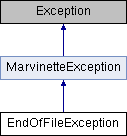
\includegraphics[height=3.000000cm]{classEndOfFileException}
\end{center}
\end{figure}


\subsection{Detailed Description}
Exception class for E\+OF error 

The documentation for this class was generated from the following file\+:\begin{DoxyCompactItemize}
\item 
src/\+Exception/End\+Of\+File\+Exception.\+php\end{DoxyCompactItemize}

\hypertarget{classField}{}\section{Field Class Reference}
\label{classField}\index{Field@{Field}}


Object representing a class\textquotesingle{}s variable member, but allows error handling and prompt help messages.  


\subsection*{Public Member Functions}
\begin{DoxyCompactItemize}
\item 
\hyperlink{classField_ae052e0e3c5726e58db49bdbc1e2df358}{\+\_\+\+\_\+to\+String} ()
\item 
\hyperlink{classField_a360a1d2e980c0168004a5e2d29505995}{\+\_\+\+\_\+construct} (callable \$error\+Handler, \$data\+Cleaner=null, ?string \$prompt\+Help=null)
\begin{DoxyCompactList}\small\item\em A \hyperlink{classField}{Field} constructor, should be called in constructor of class. \end{DoxyCompactList}\item 
\hyperlink{classField_a0256105b39f3e33f4a52ec0dabca6369}{get} ()
\item 
\hyperlink{classField_a0c9ef207aaf0de57c8f4a0a96a25d5e4}{set} (\$data)
\begin{DoxyCompactList}\small\item\em Call the error handler, with no exception handling If a data cleaner is set, the value retuend by this function will be set to {\ttfamily \$data} {\ttfamily \$data} is set to the object\textquotesingle{}s data field. \end{DoxyCompactList}\item 
\hyperlink{classField_a0a70ba06268a998a95875ab373c981c8}{get\+Prompt\+Help} ()
\end{DoxyCompactItemize}
\subsection*{Static Public Member Functions}
\begin{DoxyCompactItemize}
\item 
static \hyperlink{classField_a1264ea9bdc12d6d5b6e6189508276ebb}{Yes\+No\+Error\+Handler} (\$choice)
\item 
static \hyperlink{classField_a5f84b56e8ea34c9b15081751366392c8}{Yes\+No\+Data\+Cleaner} (\$choice)
\item 
static \hyperlink{classField_aae2d2da0cdb35adf97d9a83664613b7d}{Empty\+Data\+Cleaner} (\$input)
\end{DoxyCompactItemize}
\subsection*{Protected Attributes}
\begin{DoxyCompactItemize}
\item 
\mbox{\Hypertarget{classField_a4ef2767bbc9edafc28b43fcafc9cfc14}\label{classField_a4ef2767bbc9edafc28b43fcafc9cfc14}} 
{\bfseries \$data} = null
\item 
\mbox{\Hypertarget{classField_ab99fddcf18839cfba9038b7ca5cb0505}\label{classField_ab99fddcf18839cfba9038b7ca5cb0505}} 
{\bfseries \$error\+Handler}
\item 
\mbox{\Hypertarget{classField_af12f4a8d51558e1e41cfd7aaed5a5e5e}\label{classField_af12f4a8d51558e1e41cfd7aaed5a5e5e}} 
{\bfseries \$data\+Cleaner}
\item 
\mbox{\Hypertarget{classField_aec8b430e3b1f483094a122f89a657470}\label{classField_aec8b430e3b1f483094a122f89a657470}} 
string {\bfseries \$prompt\+Help} = null
\end{DoxyCompactItemize}


\subsection{Detailed Description}
Object representing a class\textquotesingle{}s variable member, but allows error handling and prompt help messages. 

\subsection{Constructor \& Destructor Documentation}
\mbox{\Hypertarget{classField_a360a1d2e980c0168004a5e2d29505995}\label{classField_a360a1d2e980c0168004a5e2d29505995}} 
\index{Field@{Field}!\+\_\+\+\_\+construct@{\+\_\+\+\_\+construct}}
\index{\+\_\+\+\_\+construct@{\+\_\+\+\_\+construct}!Field@{Field}}
\subsubsection{\texorpdfstring{\+\_\+\+\_\+construct()}{\_\_construct()}}
{\footnotesize\ttfamily Field\+::\+\_\+\+\_\+construct (\begin{DoxyParamCaption}\item[{callable}]{\$error\+Handler,  }\item[{}]{\$data\+Cleaner = {\ttfamily null},  }\item[{?string}]{\$prompt\+Help = {\ttfamily null} }\end{DoxyParamCaption})}



A \hyperlink{classField}{Field} constructor, should be called in constructor of class. 


\begin{DoxyParams}[1]{Parameters}
callable & {\em \$error\+Handler} & the function to handle error\+: must throw when error occurs (will be called using call\+\_\+user\+\_\+func) \\
\hline
callable & {\em \$datacleaner} & the function to clean the data (can be null) (will be called using call\+\_\+user\+\_\+func) \\
\hline
string & {\em \$prompt\+Help} & a help message, which will be displayed when the user is prompted to type the field \\
\hline
\end{DoxyParams}


\subsection{Member Function Documentation}
\mbox{\Hypertarget{classField_ae052e0e3c5726e58db49bdbc1e2df358}\label{classField_ae052e0e3c5726e58db49bdbc1e2df358}} 
\index{Field@{Field}!\+\_\+\+\_\+to\+String@{\+\_\+\+\_\+to\+String}}
\index{\+\_\+\+\_\+to\+String@{\+\_\+\+\_\+to\+String}!Field@{Field}}
\subsubsection{\texorpdfstring{\+\_\+\+\_\+to\+String()}{\_\_toString()}}
{\footnotesize\ttfamily Field\+::\+\_\+\+\_\+to\+String (\begin{DoxyParamCaption}{ }\end{DoxyParamCaption})}

Converts data to string when possible Avoid using {\ttfamily get} getter method \begin{DoxyReturn}{Returns}
string 
\end{DoxyReturn}
\mbox{\Hypertarget{classField_aae2d2da0cdb35adf97d9a83664613b7d}\label{classField_aae2d2da0cdb35adf97d9a83664613b7d}} 
\index{Field@{Field}!Empty\+Data\+Cleaner@{Empty\+Data\+Cleaner}}
\index{Empty\+Data\+Cleaner@{Empty\+Data\+Cleaner}!Field@{Field}}
\subsubsection{\texorpdfstring{Empty\+Data\+Cleaner()}{EmptyDataCleaner()}}
{\footnotesize\ttfamily static Field\+::\+Empty\+Data\+Cleaner (\begin{DoxyParamCaption}\item[{}]{\$input }\end{DoxyParamCaption})\hspace{0.3cm}{\ttfamily [static]}}

Fata cleaner function If the user entered an empty line, the data will be set to null 
\begin{DoxyParams}[1]{Parameters}
string & {\em \$input} & a string entered by the user \\
\hline
\end{DoxyParams}
\begin{DoxyReturn}{Returns}
string$\vert$null 
\end{DoxyReturn}
\mbox{\Hypertarget{classField_a0256105b39f3e33f4a52ec0dabca6369}\label{classField_a0256105b39f3e33f4a52ec0dabca6369}} 
\index{Field@{Field}!get@{get}}
\index{get@{get}!Field@{Field}}
\subsubsection{\texorpdfstring{get()}{get()}}
{\footnotesize\ttfamily Field\+::get (\begin{DoxyParamCaption}{ }\end{DoxyParamCaption})}

Get the value of data

\begin{DoxyReturn}{Returns}
mixed 
\end{DoxyReturn}
\mbox{\Hypertarget{classField_a0a70ba06268a998a95875ab373c981c8}\label{classField_a0a70ba06268a998a95875ab373c981c8}} 
\index{Field@{Field}!get\+Prompt\+Help@{get\+Prompt\+Help}}
\index{get\+Prompt\+Help@{get\+Prompt\+Help}!Field@{Field}}
\subsubsection{\texorpdfstring{get\+Prompt\+Help()}{getPromptHelp()}}
{\footnotesize\ttfamily Field\+::get\+Prompt\+Help (\begin{DoxyParamCaption}{ }\end{DoxyParamCaption})}

Get prompt helper

\begin{DoxyReturn}{Returns}
?string 
\end{DoxyReturn}
\mbox{\Hypertarget{classField_a0c9ef207aaf0de57c8f4a0a96a25d5e4}\label{classField_a0c9ef207aaf0de57c8f4a0a96a25d5e4}} 
\index{Field@{Field}!set@{set}}
\index{set@{set}!Field@{Field}}
\subsubsection{\texorpdfstring{set()}{set()}}
{\footnotesize\ttfamily Field\+::set (\begin{DoxyParamCaption}\item[{}]{\$data }\end{DoxyParamCaption})}



Call the error handler, with no exception handling If a data cleaner is set, the value retuend by this function will be set to {\ttfamily \$data} {\ttfamily \$data} is set to the object\textquotesingle{}s data field. 


\begin{DoxyParams}[1]{Parameters}
mixed & {\em \$data} & a value entered by the user \\
\hline
\end{DoxyParams}
\begin{DoxyReturn}{Returns}
void 
\end{DoxyReturn}
\mbox{\Hypertarget{classField_a5f84b56e8ea34c9b15081751366392c8}\label{classField_a5f84b56e8ea34c9b15081751366392c8}} 
\index{Field@{Field}!Yes\+No\+Data\+Cleaner@{Yes\+No\+Data\+Cleaner}}
\index{Yes\+No\+Data\+Cleaner@{Yes\+No\+Data\+Cleaner}!Field@{Field}}
\subsubsection{\texorpdfstring{Yes\+No\+Data\+Cleaner()}{YesNoDataCleaner()}}
{\footnotesize\ttfamily static Field\+::\+Yes\+No\+Data\+Cleaner (\begin{DoxyParamCaption}\item[{}]{\$choice }\end{DoxyParamCaption})\hspace{0.3cm}{\ttfamily [static]}}

Data cleaner function If \$choice is a \textquotesingle{}yes\textquotesingle{} option string, the function returns true 
\begin{DoxyParams}[1]{Parameters}
string & {\em \$choice} & a string entered by the user \\
\hline
\end{DoxyParams}
\begin{DoxyReturn}{Returns}
bool 
\end{DoxyReturn}
\mbox{\Hypertarget{classField_a1264ea9bdc12d6d5b6e6189508276ebb}\label{classField_a1264ea9bdc12d6d5b6e6189508276ebb}} 
\index{Field@{Field}!Yes\+No\+Error\+Handler@{Yes\+No\+Error\+Handler}}
\index{Yes\+No\+Error\+Handler@{Yes\+No\+Error\+Handler}!Field@{Field}}
\subsubsection{\texorpdfstring{Yes\+No\+Error\+Handler()}{YesNoErrorHandler()}}
{\footnotesize\ttfamily static Field\+::\+Yes\+No\+Error\+Handler (\begin{DoxyParamCaption}\item[{}]{\$choice }\end{DoxyParamCaption})\hspace{0.3cm}{\ttfamily [static]}}

Error handler for object\textquotesingle{}s field Throws an exception if \$choice is not a valid \textquotesingle{}yes\textquotesingle{}/\textquotesingle{}no\textquotesingle{} string 
\begin{DoxyParams}[1]{Parameters}
string & {\em \$choice} & a string entered by the user \\
\hline
\end{DoxyParams}
\begin{DoxyReturn}{Returns}
void 
\end{DoxyReturn}


The documentation for this class was generated from the following file\+:\begin{DoxyCompactItemize}
\item 
src/Field.\+php\end{DoxyCompactItemize}

\hypertarget{classFileManager}{}\section{File\+Manager Class Reference}
\label{classFileManager}\index{File\+Manager@{File\+Manager}}
\subsection*{Static Public Member Functions}
\begin{DoxyCompactItemize}
\item 
static \hyperlink{classFileManager_a19dfbed0b7597c61ccf94fa42abae688}{delete\+Folder} (string \$folder\+Path)
\item 
static \hyperlink{classFileManager_a455adf5b72c5068e606a1e1fdb67a97e}{normalize\+Path} (string \$path)
\item 
static \hyperlink{classFileManager_afe8493bc18be1fd7d7d431142c85008e}{remove\+End\+Dir\+Separator} (string \$path)
\end{DoxyCompactItemize}


\subsection{Member Function Documentation}
\mbox{\Hypertarget{classFileManager_a19dfbed0b7597c61ccf94fa42abae688}\label{classFileManager_a19dfbed0b7597c61ccf94fa42abae688}} 
\index{File\+Manager@{File\+Manager}!delete\+Folder@{delete\+Folder}}
\index{delete\+Folder@{delete\+Folder}!File\+Manager@{File\+Manager}}
\subsubsection{\texorpdfstring{delete\+Folder()}{deleteFolder()}}
{\footnotesize\ttfamily static File\+Manager\+::delete\+Folder (\begin{DoxyParamCaption}\item[{string}]{\$folder\+Path }\end{DoxyParamCaption})\hspace{0.3cm}{\ttfamily [static]}}

Deletes a folder, and its content 
\begin{DoxyParams}[1]{Parameters}
string & {\em \$folder\+Path} & the full or relative path to a folder \\
\hline
\end{DoxyParams}
\begin{DoxyReturn}{Returns}
void 
\end{DoxyReturn}
\mbox{\Hypertarget{classFileManager_a455adf5b72c5068e606a1e1fdb67a97e}\label{classFileManager_a455adf5b72c5068e606a1e1fdb67a97e}} 
\index{File\+Manager@{File\+Manager}!normalize\+Path@{normalize\+Path}}
\index{normalize\+Path@{normalize\+Path}!File\+Manager@{File\+Manager}}
\subsubsection{\texorpdfstring{normalize\+Path()}{normalizePath()}}
{\footnotesize\ttfamily static File\+Manager\+::normalize\+Path (\begin{DoxyParamCaption}\item[{string}]{\$path }\end{DoxyParamCaption})\hspace{0.3cm}{\ttfamily [static]}}

replace every backslashes and forwardslashes with D\+I\+R\+E\+C\+T\+O\+R\+Y\+\_\+\+S\+E\+P\+A\+R\+A\+T\+OR t oobtain cross-\/platform path 
\begin{DoxyParams}[1]{Parameters}
string & {\em \$path} & a file path containing directory separators \\
\hline
\end{DoxyParams}
\begin{DoxyReturn}{Returns}
string 
\end{DoxyReturn}
\mbox{\Hypertarget{classFileManager_afe8493bc18be1fd7d7d431142c85008e}\label{classFileManager_afe8493bc18be1fd7d7d431142c85008e}} 
\index{File\+Manager@{File\+Manager}!remove\+End\+Dir\+Separator@{remove\+End\+Dir\+Separator}}
\index{remove\+End\+Dir\+Separator@{remove\+End\+Dir\+Separator}!File\+Manager@{File\+Manager}}
\subsubsection{\texorpdfstring{remove\+End\+Dir\+Separator()}{removeEndDirSeparator()}}
{\footnotesize\ttfamily static File\+Manager\+::remove\+End\+Dir\+Separator (\begin{DoxyParamCaption}\item[{string}]{\$path }\end{DoxyParamCaption})\hspace{0.3cm}{\ttfamily [static]}}

Remove last character if it is a directory separator 
\begin{DoxyParams}[1]{Parameters}
string & {\em \$ath} & a filepath \\
\hline
\end{DoxyParams}


The documentation for this class was generated from the following file\+:\begin{DoxyCompactItemize}
\item 
src/\+Utils/File\+Manager.\+php\end{DoxyCompactItemize}

\hypertarget{classInvalidConfigFileException}{}\section{Invalid\+Config\+File\+Exception Class Reference}
\label{classInvalidConfigFileException}\index{Invalid\+Config\+File\+Exception@{Invalid\+Config\+File\+Exception}}
Inheritance diagram for Invalid\+Config\+File\+Exception\+:\begin{figure}[H]
\begin{center}
\leavevmode
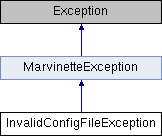
\includegraphics[height=3.000000cm]{classInvalidConfigFileException}
\end{center}
\end{figure}


\subsection{Detailed Description}
Exception class for test folder errors 

The documentation for this class was generated from the following file\+:\begin{DoxyCompactItemize}
\item 
src/\+Exception/Invalid\+Config\+File\+Exception.\+php\end{DoxyCompactItemize}

\hypertarget{classInvalidTestFolderException}{}\section{Invalid\+Test\+Folder\+Exception Class Reference}
\label{classInvalidTestFolderException}\index{Invalid\+Test\+Folder\+Exception@{Invalid\+Test\+Folder\+Exception}}
Inheritance diagram for Invalid\+Test\+Folder\+Exception\+:\begin{figure}[H]
\begin{center}
\leavevmode
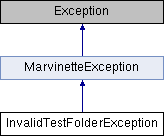
\includegraphics[height=3.000000cm]{classInvalidTestFolderException}
\end{center}
\end{figure}


\subsection{Detailed Description}
Exception class for test folder errors 

The documentation for this class was generated from the following file\+:\begin{DoxyCompactItemize}
\item 
src/\+Exception/Invalid\+Test\+Folder\+Exception.\+php\end{DoxyCompactItemize}

\hypertarget{classMarvinetteException}{}\section{Marvinette\+Exception Class Reference}
\label{classMarvinetteException}\index{Marvinette\+Exception@{Marvinette\+Exception}}
Inheritance diagram for Marvinette\+Exception\+:\begin{figure}[H]
\begin{center}
\leavevmode
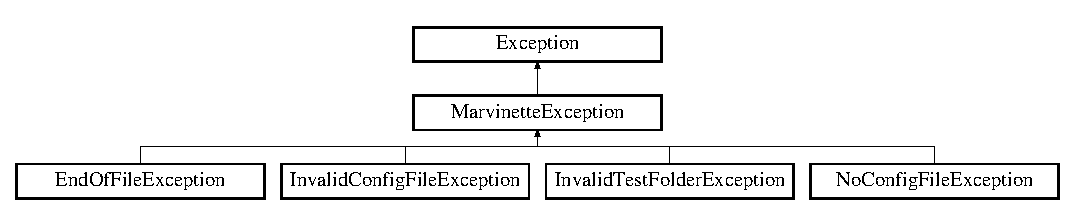
\includegraphics[height=2.441860cm]{classMarvinetteException}
\end{center}
\end{figure}


\subsection{Detailed Description}
Base class for exceptions 

The documentation for this class was generated from the following file\+:\begin{DoxyCompactItemize}
\item 
src/\+Exception/Marvinette\+Exception.\+php\end{DoxyCompactItemize}

\hypertarget{classNoConfigFileException}{}\section{No\+Config\+File\+Exception Class Reference}
\label{classNoConfigFileException}\index{No\+Config\+File\+Exception@{No\+Config\+File\+Exception}}
Inheritance diagram for No\+Config\+File\+Exception\+:\begin{figure}[H]
\begin{center}
\leavevmode
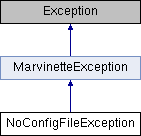
\includegraphics[height=3.000000cm]{classNoConfigFileException}
\end{center}
\end{figure}


\subsection{Detailed Description}
Exception class for test folder errors 

The documentation for this class was generated from the following file\+:\begin{DoxyCompactItemize}
\item 
src/\+Exception/No\+Config\+File\+Exception.\+php\end{DoxyCompactItemize}

\hypertarget{classObjectHelper}{}\section{Object\+Helper Class Reference}
\label{classObjectHelper}\index{Object\+Helper@{Object\+Helper}}
\subsection*{Static Public Member Functions}
\begin{DoxyCompactItemize}
\item 
static \hyperlink{classObjectHelper_ac4635dabbe7d6552d0bc6c3bcb2da485}{for\+Each\+Object\+Field} (\&\$obj, callable \$callable)
\item 
static \hyperlink{classObjectHelper_aee0184a88585f2872a33f0311cfe1457}{prompt\+Each\+Object\+Field} (\&\$obj, callable \$display\+Prompt, bool \$mod\+Prompt=false, array \$ignored\+Fields=\mbox{[}$\,$\mbox{]})
\end{DoxyCompactItemize}


\subsection{Detailed Description}
Set of function which help iterate through object\textquotesingle{}s fields 

\subsection{Member Function Documentation}
\mbox{\Hypertarget{classObjectHelper_ac4635dabbe7d6552d0bc6c3bcb2da485}\label{classObjectHelper_ac4635dabbe7d6552d0bc6c3bcb2da485}} 
\index{Object\+Helper@{Object\+Helper}!for\+Each\+Object\+Field@{for\+Each\+Object\+Field}}
\index{for\+Each\+Object\+Field@{for\+Each\+Object\+Field}!Object\+Helper@{Object\+Helper}}
\subsubsection{\texorpdfstring{for\+Each\+Object\+Field()}{forEachObjectField()}}
{\footnotesize\ttfamily static Object\+Helper\+::for\+Each\+Object\+Field (\begin{DoxyParamCaption}\item[{\&}]{\$obj,  }\item[{callable}]{\$callable }\end{DoxyParamCaption})\hspace{0.3cm}{\ttfamily [static]}}

Calls \$callable on each field of \$obj 
\begin{DoxyParams}[1]{Parameters}
callable & {\em \$callable} & a function taking 2 parameters\+: a string being the field\textquotesingle{}s nameand the field object. retusn true on success, false on error, null on fatal error \\
\hline
object & {\em \$obj} & a refence to an object \\
\hline
\end{DoxyParams}
\begin{DoxyReturn}{Returns}
bool true if everything succeeded 
\end{DoxyReturn}
\mbox{\Hypertarget{classObjectHelper_aee0184a88585f2872a33f0311cfe1457}\label{classObjectHelper_aee0184a88585f2872a33f0311cfe1457}} 
\index{Object\+Helper@{Object\+Helper}!prompt\+Each\+Object\+Field@{prompt\+Each\+Object\+Field}}
\index{prompt\+Each\+Object\+Field@{prompt\+Each\+Object\+Field}!Object\+Helper@{Object\+Helper}}
\subsubsection{\texorpdfstring{prompt\+Each\+Object\+Field()}{promptEachObjectField()}}
{\footnotesize\ttfamily static Object\+Helper\+::prompt\+Each\+Object\+Field (\begin{DoxyParamCaption}\item[{\&}]{\$obj,  }\item[{callable}]{\$display\+Prompt,  }\item[{bool}]{\$mod\+Prompt = {\ttfamily false},  }\item[{array}]{\$ignored\+Fields = {\ttfamily \mbox{[}\mbox{]}} }\end{DoxyParamCaption})\hspace{0.3cm}{\ttfamily [static]}}

Prompt user to enter each obbjec\textquotesingle{}s field 
\begin{DoxyParams}[1]{Parameters}
object & {\em \$obj} & the object to iterate through \\
\hline
callable & {\em \$prompt\+Formatter} & a function that display prompt using field\textquotesingle{}s name and field \\
\hline
bool & {\em \$mod\+Prompt} & if true and value entered is empty, the old value is not modified \\
\hline
array & {\em \$ignored\+Fields} & an array of string containing fields\textquotesingle{} names that will be ingore at prompt \\
\hline
\end{DoxyParams}


The documentation for this class was generated from the following file\+:\begin{DoxyCompactItemize}
\item 
src/\+Utils/Object\+Helper.\+php\end{DoxyCompactItemize}

\hypertarget{classProject}{}\section{Project Class Reference}
\label{classProject}\index{Project@{Project}}


Object representing the project\textquotesingle{}s important infos.  


\subsection*{Public Member Functions}
\begin{DoxyCompactItemize}
\item 
\hyperlink{classProject_a8cdc8d54b71a7084cd0ed8f30fbec1bc}{\+\_\+\+\_\+construct} (?string \$file\+Path=null)
\item 
\hyperlink{classProject_ae494148807f65c817af1e3b0139fee5f}{ready\+To\+Export} ()
\item 
\hyperlink{classProject_aba3771ee0f7928f720510eea8a6b3337}{build\+Binary\+Access\+Path} ()
\item 
\hyperlink{classProject_a96804c40f63ec38018f480c73a7c20a8}{interpreter\+Exists} ()
\item 
\hyperlink{classProject_ab08a24e761958ef13b631cb5155286ad}{get\+Interpreter\+Full\+Path} ()
\item 
\hyperlink{classProject_a290cf05d80192d6ea99c119e91631197}{is\+Ready\+To\+Be\+Tested} ()
\item 
\hyperlink{classProject_af50a24af7524ef28c4d7b39f53153498}{export} (string \$outfile)
\item 
\hyperlink{classProject_a726e3f6542b4b4a15c8c73f92fa84b5a}{import} (string \$infile)
\end{DoxyCompactItemize}
\subsection*{Static Public Member Functions}
\begin{DoxyCompactItemize}
\item 
static \hyperlink{classProject_a5c9ad606315d82f9d09c5fef29b930e2}{export\+Sample} ()
\end{DoxyCompactItemize}
\subsection*{Public Attributes}
\begin{DoxyCompactItemize}
\item 
\mbox{\Hypertarget{classProject_af24a2186c2669ac5acfa29fbc71c7bd2}\label{classProject_af24a2186c2669ac5acfa29fbc71c7bd2}} 
const {\bfseries Configuration\+File} = \char`\"{}Marvinette.\+json\char`\"{}
\item 
\mbox{\Hypertarget{classProject_abf56709b7a46b62d9d7febddad179197}\label{classProject_abf56709b7a46b62d9d7febddad179197}} 
\hyperlink{classField}{Field} {\bfseries \$name}
\item 
\mbox{\Hypertarget{classProject_a3b8e966f7165ec5e6df102679eab5bbc}\label{classProject_a3b8e966f7165ec5e6df102679eab5bbc}} 
\hyperlink{classField}{Field} {\bfseries \$binary\+Name}
\item 
\mbox{\Hypertarget{classProject_a010db9bfd82fd07c825f26910b5b1953}\label{classProject_a010db9bfd82fd07c825f26910b5b1953}} 
\hyperlink{classField}{Field} {\bfseries \$binary\+Path}
\item 
\mbox{\Hypertarget{classProject_a410292d6310de22b8404b5128892b3cc}\label{classProject_a410292d6310de22b8404b5128892b3cc}} 
\hyperlink{classField}{Field} {\bfseries \$interpreter}
\item 
\mbox{\Hypertarget{classProject_a31ff999c516ebcbe9103b16eeb73bf5f}\label{classProject_a31ff999c516ebcbe9103b16eeb73bf5f}} 
\hyperlink{classField}{Field} {\bfseries \$tests\+Folder}
\end{DoxyCompactItemize}


\subsection{Detailed Description}
Object representing the project\textquotesingle{}s important infos. 

\subsection{Constructor \& Destructor Documentation}
\mbox{\Hypertarget{classProject_a8cdc8d54b71a7084cd0ed8f30fbec1bc}\label{classProject_a8cdc8d54b71a7084cd0ed8f30fbec1bc}} 
\index{Project@{Project}!\+\_\+\+\_\+construct@{\+\_\+\+\_\+construct}}
\index{\+\_\+\+\_\+construct@{\+\_\+\+\_\+construct}!Project@{Project}}
\subsubsection{\texorpdfstring{\+\_\+\+\_\+construct()}{\_\_construct()}}
{\footnotesize\ttfamily Project\+::\+\_\+\+\_\+construct (\begin{DoxyParamCaption}\item[{?string}]{\$file\+Path = {\ttfamily null} }\end{DoxyParamCaption})}


\begin{DoxyParams}{Parameters}
{\em ?string} & \$file\+Path a path to a J\+S\+ON \hyperlink{classProject}{Project} file \\
\hline
\end{DoxyParams}


\subsection{Member Function Documentation}
\mbox{\Hypertarget{classProject_aba3771ee0f7928f720510eea8a6b3337}\label{classProject_aba3771ee0f7928f720510eea8a6b3337}} 
\index{Project@{Project}!build\+Binary\+Access\+Path@{build\+Binary\+Access\+Path}}
\index{build\+Binary\+Access\+Path@{build\+Binary\+Access\+Path}!Project@{Project}}
\subsubsection{\texorpdfstring{build\+Binary\+Access\+Path()}{buildBinaryAccessPath()}}
{\footnotesize\ttfamily Project\+::build\+Binary\+Access\+Path (\begin{DoxyParamCaption}{ }\end{DoxyParamCaption})}

\begin{DoxyReturn}{Returns}
string binary access path 
\end{DoxyReturn}
\mbox{\Hypertarget{classProject_af50a24af7524ef28c4d7b39f53153498}\label{classProject_af50a24af7524ef28c4d7b39f53153498}} 
\index{Project@{Project}!export@{export}}
\index{export@{export}!Project@{Project}}
\subsubsection{\texorpdfstring{export()}{export()}}
{\footnotesize\ttfamily Project\+::export (\begin{DoxyParamCaption}\item[{string}]{\$outfile }\end{DoxyParamCaption})}

Export \hyperlink{classProject}{Project} to J\+S\+ON formatted file 
\begin{DoxyParams}{Parameters}
{\em \$outfile} & name of file with J\+S\+O\+N-\/ed \hyperlink{classProject}{Project} class \\
\hline
\end{DoxyParams}
\mbox{\Hypertarget{classProject_a5c9ad606315d82f9d09c5fef29b930e2}\label{classProject_a5c9ad606315d82f9d09c5fef29b930e2}} 
\index{Project@{Project}!export\+Sample@{export\+Sample}}
\index{export\+Sample@{export\+Sample}!Project@{Project}}
\subsubsection{\texorpdfstring{export\+Sample()}{exportSample()}}
{\footnotesize\ttfamily static Project\+::export\+Sample (\begin{DoxyParamCaption}{ }\end{DoxyParamCaption})\hspace{0.3cm}{\ttfamily [static]}}

Exports to Marvinette.\+json an empty configation structure \mbox{\Hypertarget{classProject_ab08a24e761958ef13b631cb5155286ad}\label{classProject_ab08a24e761958ef13b631cb5155286ad}} 
\index{Project@{Project}!get\+Interpreter\+Full\+Path@{get\+Interpreter\+Full\+Path}}
\index{get\+Interpreter\+Full\+Path@{get\+Interpreter\+Full\+Path}!Project@{Project}}
\subsubsection{\texorpdfstring{get\+Interpreter\+Full\+Path()}{getInterpreterFullPath()}}
{\footnotesize\ttfamily Project\+::get\+Interpreter\+Full\+Path (\begin{DoxyParamCaption}{ }\end{DoxyParamCaption})}

Using P\+A\+Th Env var, get interpreter\textquotesingle{}s full path, or null if not throw if no interpreter is set \mbox{\Hypertarget{classProject_a726e3f6542b4b4a15c8c73f92fa84b5a}\label{classProject_a726e3f6542b4b4a15c8c73f92fa84b5a}} 
\index{Project@{Project}!import@{import}}
\index{import@{import}!Project@{Project}}
\subsubsection{\texorpdfstring{import()}{import()}}
{\footnotesize\ttfamily Project\+::import (\begin{DoxyParamCaption}\item[{string}]{\$infile }\end{DoxyParamCaption})}

Fills the object\textquotesingle{}s field using json file 
\begin{DoxyParams}[1]{Parameters}
string & {\em \$infile} & the path to a valid J\+S\+ON \hyperlink{classProject}{Project} file \\
\hline
\end{DoxyParams}
\mbox{\Hypertarget{classProject_a96804c40f63ec38018f480c73a7c20a8}\label{classProject_a96804c40f63ec38018f480c73a7c20a8}} 
\index{Project@{Project}!interpreter\+Exists@{interpreter\+Exists}}
\index{interpreter\+Exists@{interpreter\+Exists}!Project@{Project}}
\subsubsection{\texorpdfstring{interpreter\+Exists()}{interpreterExists()}}
{\footnotesize\ttfamily Project\+::interpreter\+Exists (\begin{DoxyParamCaption}{ }\end{DoxyParamCaption})}

Using P\+A\+Th Env var, checks if interpreter exists throw if no interpreter is set \mbox{\Hypertarget{classProject_a290cf05d80192d6ea99c119e91631197}\label{classProject_a290cf05d80192d6ea99c119e91631197}} 
\index{Project@{Project}!is\+Ready\+To\+Be\+Tested@{is\+Ready\+To\+Be\+Tested}}
\index{is\+Ready\+To\+Be\+Tested@{is\+Ready\+To\+Be\+Tested}!Project@{Project}}
\subsubsection{\texorpdfstring{is\+Ready\+To\+Be\+Tested()}{isReadyToBeTested()}}
{\footnotesize\ttfamily Project\+::is\+Ready\+To\+Be\+Tested (\begin{DoxyParamCaption}{ }\end{DoxyParamCaption})}

Checks if the binary exists the interpreter exists (if set) (need to be ready to export) \mbox{\Hypertarget{classProject_ae494148807f65c817af1e3b0139fee5f}\label{classProject_ae494148807f65c817af1e3b0139fee5f}} 
\index{Project@{Project}!ready\+To\+Export@{ready\+To\+Export}}
\index{ready\+To\+Export@{ready\+To\+Export}!Project@{Project}}
\subsubsection{\texorpdfstring{ready\+To\+Export()}{readyToExport()}}
{\footnotesize\ttfamily Project\+::ready\+To\+Export (\begin{DoxyParamCaption}{ }\end{DoxyParamCaption})}

\begin{DoxyReturn}{Returns}
bool true if all necessary fields are set interpreter can be null 
\end{DoxyReturn}


The documentation for this class was generated from the following file\+:\begin{DoxyCompactItemize}
\item 
src/Project.\+php\end{DoxyCompactItemize}

\hypertarget{classProjectManager}{}\section{Project\+Manager Class Reference}
\label{classProjectManager}\index{Project\+Manager@{Project\+Manager}}
\subsection*{Static Public Member Functions}
\begin{DoxyCompactItemize}
\item 
\mbox{\Hypertarget{classProjectManager_afa4ee771ac7d6da3e4b76779745ebcfa}\label{classProjectManager_afa4ee771ac7d6da3e4b76779745ebcfa}} 
static {\bfseries create\+Project} ()
\item 
\mbox{\Hypertarget{classProjectManager_af594dfa22322495cf15c5c47078a3eef}\label{classProjectManager_af594dfa22322495cf15c5c47078a3eef}} 
static {\bfseries create\+Sample\+Project} ()
\item 
\mbox{\Hypertarget{classProjectManager_a05c781c75177c7f9165cde755220e7e1}\label{classProjectManager_a05c781c75177c7f9165cde755220e7e1}} 
static {\bfseries prompt\+Add\+Test} ()
\item 
\mbox{\Hypertarget{classProjectManager_a7eae0be214d994ccb4d8f732079f40bf}\label{classProjectManager_a7eae0be214d994ccb4d8f732079f40bf}} 
static {\bfseries display\+No\+Config\+File\+Found} ()
\item 
\mbox{\Hypertarget{classProjectManager_ae22d0ea1ed86b8ba48478e3d25553032}\label{classProjectManager_ae22d0ea1ed86b8ba48478e3d25553032}} 
static {\bfseries mod\+Project} ()
\item 
\mbox{\Hypertarget{classProjectManager_af29d3ef5fceb1c2b6ac66596210b82d7}\label{classProjectManager_af29d3ef5fceb1c2b6ac66596210b82d7}} 
static {\bfseries delete\+Project} ()
\item 
\mbox{\Hypertarget{classProjectManager_a25b38d08f39666c093ef226557011d9e}\label{classProjectManager_a25b38d08f39666c093ef226557011d9e}} 
static {\bfseries prompt\+Overwrite\+Project} ()
\end{DoxyCompactItemize}


\subsection{Detailed Description}
Object holding method where the main functions are 

The documentation for this class was generated from the following file\+:\begin{DoxyCompactItemize}
\item 
src/Project\+Manager.\+php\end{DoxyCompactItemize}

\hypertarget{classDisplay_1_1Style}{}\section{Display\textbackslash{}Style Class Reference}
\label{classDisplay_1_1Style}\index{Display\textbackslash{}\+Style@{Display\textbackslash{}\+Style}}


static class holding style int for terminal display  


\subsection*{Public Attributes}
\begin{DoxyCompactItemize}
\item 
\mbox{\Hypertarget{classDisplay_1_1Style_a2c069acaa67c5efdd7821e4b2d71d472}\label{classDisplay_1_1Style_a2c069acaa67c5efdd7821e4b2d71d472}} 
const \hyperlink{classDisplay_1_1Style_a2c069acaa67c5efdd7821e4b2d71d472}{Default} = 0
\begin{DoxyCompactList}\small\item\em id letting the terminal know to write using default style \end{DoxyCompactList}\item 
\mbox{\Hypertarget{classDisplay_1_1Style_a26273dd8c98b09d0d7ffe0eef7583a87}\label{classDisplay_1_1Style_a26273dd8c98b09d0d7ffe0eef7583a87}} 
const \hyperlink{classDisplay_1_1Style_a26273dd8c98b09d0d7ffe0eef7583a87}{Bold} = 1
\begin{DoxyCompactList}\small\item\em id letting the terminal know to write in bold \end{DoxyCompactList}\item 
\mbox{\Hypertarget{classDisplay_1_1Style_a78cb8aef7afff0bde92008d9a216e1c2}\label{classDisplay_1_1Style_a78cb8aef7afff0bde92008d9a216e1c2}} 
const \hyperlink{classDisplay_1_1Style_a78cb8aef7afff0bde92008d9a216e1c2}{Dim} = 2
\begin{DoxyCompactList}\small\item\em id letting the terminal know to write in dim \end{DoxyCompactList}\item 
\mbox{\Hypertarget{classDisplay_1_1Style_a381dbe5a47d442953744e252f2e1c2ec}\label{classDisplay_1_1Style_a381dbe5a47d442953744e252f2e1c2ec}} 
const \hyperlink{classDisplay_1_1Style_a381dbe5a47d442953744e252f2e1c2ec}{Underlined} = 4
\begin{DoxyCompactList}\small\item\em id letting the terminal know to write underlined \end{DoxyCompactList}\item 
\mbox{\Hypertarget{classDisplay_1_1Style_a0c232b5dbf81b4ffcba9e134b8751166}\label{classDisplay_1_1Style_a0c232b5dbf81b4ffcba9e134b8751166}} 
const \hyperlink{classDisplay_1_1Style_a0c232b5dbf81b4ffcba9e134b8751166}{Blink} = 5
\begin{DoxyCompactList}\small\item\em id letting the terminal know to write and blink \end{DoxyCompactList}\item 
\mbox{\Hypertarget{classDisplay_1_1Style_ab675eae45b0ec96048c51f4cf015b615}\label{classDisplay_1_1Style_ab675eae45b0ec96048c51f4cf015b615}} 
const \hyperlink{classDisplay_1_1Style_ab675eae45b0ec96048c51f4cf015b615}{Reverse\+Fore\+Back} = 7
\begin{DoxyCompactList}\small\item\em id letting the terminal know to write and invert foreground and background \end{DoxyCompactList}\item 
\mbox{\Hypertarget{classDisplay_1_1Style_acbb70d4c7fe1bef0445f4775c32195d7}\label{classDisplay_1_1Style_acbb70d4c7fe1bef0445f4775c32195d7}} 
const \hyperlink{classDisplay_1_1Style_acbb70d4c7fe1bef0445f4775c32195d7}{Hidden} = 5
\begin{DoxyCompactList}\small\item\em id letting the terminal know to write and hide \end{DoxyCompactList}\end{DoxyCompactItemize}


\subsection{Detailed Description}
static class holding style int for terminal display 

The documentation for this class was generated from the following file\+:\begin{DoxyCompactItemize}
\item 
src/\+Display/Style.\+php\end{DoxyCompactItemize}

\hypertarget{classTest}{}\section{Test Class Reference}
\label{classTest}\index{Test@{Test}}


Object representing the test\textquotesingle{}s instruction.  


\subsection*{Public Member Functions}
\begin{DoxyCompactItemize}
\item 
\mbox{\Hypertarget{classTest_acf599531126e1b40f3529405e147ecfa}\label{classTest_acf599531126e1b40f3529405e147ecfa}} 
{\bfseries \+\_\+\+\_\+construct} (?string \$test\+Path=null)
\item 
\hyperlink{classTest_a61e3ace38fd982cc3b066c2ab93eb33a}{export} (string \$tests\+Folder)
\item 
\hyperlink{classTest_ab1460ff08b4bc23fe5a01b5afcc18dd2}{import} (string \$test\+Folder)
\begin{DoxyCompactList}\small\item\em import test from file in folder \end{DoxyCompactList}\item 
\hyperlink{classTest_afd7151c1c51e71d95d814b379e0947cd}{execute} (\hyperlink{classProject}{Project} \$project)
\end{DoxyCompactItemize}
\subsection*{Static Public Member Functions}
\begin{DoxyCompactItemize}
\item 
\mbox{\Hypertarget{classTest_a00189b0d67cee24b1f55ffcf2aa841bf}\label{classTest_a00189b0d67cee24b1f55ffcf2aa841bf}} 
static {\bfseries export\+Sample} (string \$tests\+Folder, string \$name)
\end{DoxyCompactItemize}
\subsection*{Public Attributes}
\begin{DoxyCompactItemize}
\item 
\mbox{\Hypertarget{classTest_af26d84c2c2033fdbdd33eaf85c67c0ea}\label{classTest_af26d84c2c2033fdbdd33eaf85c67c0ea}} 
const {\bfseries Config\+File} = \textquotesingle{}config.\+json\textquotesingle{}
\item 
\mbox{\Hypertarget{classTest_ae1b59bffc7abfa6aa0f85566b410def5}\label{classTest_ae1b59bffc7abfa6aa0f85566b410def5}} 
const {\bfseries Tmp\+File\+Folder} = Tmp\+File\+Folder
\item 
\mbox{\Hypertarget{classTest_ade02b87da948e70b2f55a3132928b039}\label{classTest_ade02b87da948e70b2f55a3132928b039}} 
const {\bfseries Tmp\+File\+Prefix} = \textquotesingle{}Marvinette\textquotesingle{}
\item 
\mbox{\Hypertarget{classTest_a083345e9a23e8c1eb45a2b0350e9f9dc}\label{classTest_a083345e9a23e8c1eb45a2b0350e9f9dc}} 
const {\bfseries Tmp\+File\+Stdout\+Prefix} = \textquotesingle{}Stdout\textquotesingle{}
\item 
\mbox{\Hypertarget{classTest_ad836169e38502a831a67ed44bec603d4}\label{classTest_ad836169e38502a831a67ed44bec603d4}} 
const {\bfseries Tmp\+File\+Stderr\+Prefix} = \textquotesingle{}Stderr\textquotesingle{}
\item 
\mbox{\Hypertarget{classTest_a659ffaf5e33a76f74a324a1704a453b9}\label{classTest_a659ffaf5e33a76f74a324a1704a453b9}} 
const {\bfseries Tmp\+File\+Filtered\+Prefix} = \textquotesingle{}Filtered\textquotesingle{}
\item 
\mbox{\Hypertarget{classTest_a279a9761018d06d3fc0ae670984c611b}\label{classTest_a279a9761018d06d3fc0ae670984c611b}} 
const {\bfseries Tmp\+Diff\+File\+Prefix} = \textquotesingle{}Diff\textquotesingle{}
\item 
\mbox{\Hypertarget{classTest_a73668b573223cd0a0a655955a1b78b80}\label{classTest_a73668b573223cd0a0a655955a1b78b80}} 
const {\bfseries Stream\+Fields} = \mbox{[}\textquotesingle{}expected\textquotesingle{} . self\+::\+Tmp\+File\+Stderr\+Prefix, \textquotesingle{}expected\textquotesingle{} . self\+::\+Tmp\+File\+Stdout\+Prefix, \textquotesingle{}stdinput\textquotesingle{}\mbox{]}
\item 
\mbox{\Hypertarget{classTest_a9c07752de0d3fb837da28d4a8a81beb8}\label{classTest_a9c07752de0d3fb837da28d4a8a81beb8}} 
\hyperlink{classField}{Field} {\bfseries \$name}
\item 
\mbox{\Hypertarget{classTest_a8e1e0c4ef28384dab9ed434b96b9c8e5}\label{classTest_a8e1e0c4ef28384dab9ed434b96b9c8e5}} 
\hyperlink{classField}{Field} {\bfseries \$command\+Line\+Arguments}
\item 
\mbox{\Hypertarget{classTest_a2481e3e2d064e0d447c301baa8b9cb46}\label{classTest_a2481e3e2d064e0d447c301baa8b9cb46}} 
\hyperlink{classField}{Field} {\bfseries \$interpreter\+Arguments}
\item 
\mbox{\Hypertarget{classTest_a56d12011d910b9aa40ad467b85fe1a40}\label{classTest_a56d12011d910b9aa40ad467b85fe1a40}} 
\hyperlink{classField}{Field} {\bfseries \$expected\+Return\+Code}
\item 
\mbox{\Hypertarget{classTest_a060f5bf12c22e7a4480a8a00759eea52}\label{classTest_a060f5bf12c22e7a4480a8a00759eea52}} 
\hyperlink{classField}{Field} {\bfseries \$stdout\+Filter}
\item 
\mbox{\Hypertarget{classTest_a2407a1d6086e9406c4ce4415f213ac34}\label{classTest_a2407a1d6086e9406c4ce4415f213ac34}} 
\hyperlink{classField}{Field} {\bfseries \$stderr\+Filter}
\item 
\mbox{\Hypertarget{classTest_ad01ebf52ac16148dabb9ec4ea55377bc}\label{classTest_ad01ebf52ac16148dabb9ec4ea55377bc}} 
\hyperlink{classField}{Field} {\bfseries \$stdinput}
\item 
\mbox{\Hypertarget{classTest_a64a9b3cdb03f4c3ea863b57fa3ea1d73}\label{classTest_a64a9b3cdb03f4c3ea863b57fa3ea1d73}} 
\hyperlink{classField}{Field} {\bfseries \$empty\+Env}
\item 
\mbox{\Hypertarget{classTest_a26361a14649bfc158727f160a0a1ba86}\label{classTest_a26361a14649bfc158727f160a0a1ba86}} 
\hyperlink{classField}{Field} {\bfseries \$expected\+Stdout}
\item 
\mbox{\Hypertarget{classTest_ad3f9aa30395f954146dd38e34191afea}\label{classTest_ad3f9aa30395f954146dd38e34191afea}} 
\hyperlink{classField}{Field} {\bfseries \$expected\+Stderr}
\item 
\mbox{\Hypertarget{classTest_a7f746d846f82b595b8f42cc70018843b}\label{classTest_a7f746d846f82b595b8f42cc70018843b}} 
\hyperlink{classField}{Field} {\bfseries \$setup}
\item 
\mbox{\Hypertarget{classTest_ada2e6af518692629f16df255ababf4ae}\label{classTest_ada2e6af518692629f16df255ababf4ae}} 
\hyperlink{classField}{Field} {\bfseries \$teardown}
\end{DoxyCompactItemize}
\subsection*{Protected Member Functions}
\begin{DoxyCompactItemize}
\item 
\hyperlink{classTest_a76e2356e087e341bba538fef7b30a3dc}{execute\+Test\+Command} (string \$command)
\item 
\hyperlink{classTest_ac9eac02dbbf02d982dda6b4aaf4e28fd}{execute\+System\+Command} (string \$command, ?string \$message=null, ?int \$expected\+Return\+Code=0)
\end{DoxyCompactItemize}


\subsection{Detailed Description}
Object representing the test\textquotesingle{}s instruction. 

\subsection{Member Function Documentation}
\mbox{\Hypertarget{classTest_afd7151c1c51e71d95d814b379e0947cd}\label{classTest_afd7151c1c51e71d95d814b379e0947cd}} 
\index{Test@{Test}!execute@{execute}}
\index{execute@{execute}!Test@{Test}}
\subsubsection{\texorpdfstring{execute()}{execute()}}
{\footnotesize\ttfamily Test\+::execute (\begin{DoxyParamCaption}\item[{\hyperlink{classProject}{Project}}]{\$project }\end{DoxyParamCaption})}

Executes A \hyperlink{classTest}{Test}, Throws when ann error occurs or on fail \begin{DoxyReturn}{Returns}
bool true on success 
\end{DoxyReturn}
\mbox{\Hypertarget{classTest_ac9eac02dbbf02d982dda6b4aaf4e28fd}\label{classTest_ac9eac02dbbf02d982dda6b4aaf4e28fd}} 
\index{Test@{Test}!execute\+System\+Command@{execute\+System\+Command}}
\index{execute\+System\+Command@{execute\+System\+Command}!Test@{Test}}
\subsubsection{\texorpdfstring{execute\+System\+Command()}{executeSystemCommand()}}
{\footnotesize\ttfamily Test\+::execute\+System\+Command (\begin{DoxyParamCaption}\item[{string}]{\$command,  }\item[{?string}]{\$message = {\ttfamily null},  }\item[{?int}]{\$expected\+Return\+Code = {\ttfamily 0} }\end{DoxyParamCaption})\hspace{0.3cm}{\ttfamily [protected]}}

Calls {\ttfamily system} function passing \$command as parameter If the return code differs from \$expected\+Return\+Code, throws 
\begin{DoxyParams}[1]{Parameters}
string & {\em \$command} & shell command \\
\hline
int & {\em \$expected\+Return\+Code} & If the return code differs from it, the function hrows \\
\hline
string & {\em \$message} & what the exception message should contain. The return code will be inserted after \\
\hline
\end{DoxyParams}
\mbox{\Hypertarget{classTest_a76e2356e087e341bba538fef7b30a3dc}\label{classTest_a76e2356e087e341bba538fef7b30a3dc}} 
\index{Test@{Test}!execute\+Test\+Command@{execute\+Test\+Command}}
\index{execute\+Test\+Command@{execute\+Test\+Command}!Test@{Test}}
\subsubsection{\texorpdfstring{execute\+Test\+Command()}{executeTestCommand()}}
{\footnotesize\ttfamily Test\+::execute\+Test\+Command (\begin{DoxyParamCaption}\item[{string}]{\$command }\end{DoxyParamCaption})\hspace{0.3cm}{\ttfamily [protected]}}

Execute \$command using {\ttfamily system} If the return code differs from what is expected (field expected\+Return\+Code), the function throws 
\begin{DoxyParams}[1]{Parameters}
string & {\em \$command} & the shell command to execute project\textquotesingle{}s binary \\
\hline
\end{DoxyParams}
\mbox{\Hypertarget{classTest_a61e3ace38fd982cc3b066c2ab93eb33a}\label{classTest_a61e3ace38fd982cc3b066c2ab93eb33a}} 
\index{Test@{Test}!export@{export}}
\index{export@{export}!Test@{Test}}
\subsubsection{\texorpdfstring{export()}{export()}}
{\footnotesize\ttfamily Test\+::export (\begin{DoxyParamCaption}\item[{string}]{\$tests\+Folder }\end{DoxyParamCaption})}

Will export the test in a folder placed in \$tests\+Folder` 
\begin{DoxyParams}[1]{Parameters}
string & {\em \$tests\+Folder} & the path to the folder where the test\textquotesingle{}s folder will be placed \\
\hline
\end{DoxyParams}
\mbox{\Hypertarget{classTest_ab1460ff08b4bc23fe5a01b5afcc18dd2}\label{classTest_ab1460ff08b4bc23fe5a01b5afcc18dd2}} 
\index{Test@{Test}!import@{import}}
\index{import@{import}!Test@{Test}}
\subsubsection{\texorpdfstring{import()}{import()}}
{\footnotesize\ttfamily Test\+::import (\begin{DoxyParamCaption}\item[{string}]{\$test\+Folder }\end{DoxyParamCaption})}



import test from file in folder 


\begin{DoxyParams}{Parameters}
{\em \$tests\+Folder} & the path to the test folder \\
\hline
\end{DoxyParams}


The documentation for this class was generated from the following file\+:\begin{DoxyCompactItemize}
\item 
src/Test.\+php\end{DoxyCompactItemize}

\hypertarget{classTestManager}{}\section{Test\+Manager Class Reference}
\label{classTestManager}\index{Test\+Manager@{Test\+Manager}}
\subsection*{Static Public Member Functions}
\begin{DoxyCompactItemize}
\item 
\mbox{\Hypertarget{classTestManager_aa9e3945c44816be04e329864d5a2e62f}\label{classTestManager_aa9e3945c44816be04e329864d5a2e62f}} 
static {\bfseries add\+Test} (?\hyperlink{classProject}{Project} \$project=null)
\item 
\mbox{\Hypertarget{classTestManager_aee45ea866ce32f86451843a567db9e80}\label{classTestManager_aee45ea866ce32f86451843a567db9e80}} 
static {\bfseries create\+Sample\+Test} (?string \$name=null)
\item 
\mbox{\Hypertarget{classTestManager_a3d44eb840485d2f33dee6598e0e3b0ba}\label{classTestManager_a3d44eb840485d2f33dee6598e0e3b0ba}} 
static {\bfseries mod\+Test} ()
\item 
\mbox{\Hypertarget{classTestManager_a97efdce7cd3add364637cc24a15a4c48}\label{classTestManager_a97efdce7cd3add364637cc24a15a4c48}} 
static {\bfseries execute\+Test} (?string \$test\+Name=null, ?\hyperlink{classProject}{Project} \$project=null)
\item 
\mbox{\Hypertarget{classTestManager_a4a11654c5a32e8f0ccdd582bdb3ef1fa}\label{classTestManager_a4a11654c5a32e8f0ccdd582bdb3ef1fa}} 
static {\bfseries executes\+All\+Tests} (?\hyperlink{classProject}{Project} \$project=null)
\item 
\mbox{\Hypertarget{classTestManager_a19a87ea290be92044cea0d5606541c37}\label{classTestManager_a19a87ea290be92044cea0d5606541c37}} 
static {\bfseries delete\+Test} ()
\item 
static \hyperlink{classTestManager_a0f62639ed81588be321cafc0a23ac290}{folder\+Is\+A\+Test} (string \$path)
\item 
static \hyperlink{classTestManager_aa6ec0809a03f384869c41f51507a2fd4}{get\+Tests\+Folders} (string \$tests\+Folder, bool \$full\+Path=false)
\item 
\mbox{\Hypertarget{classTestManager_ad9a11b0c53f20112d0685e4700fcfa12}\label{classTestManager_ad9a11b0c53f20112d0685e4700fcfa12}} 
static {\bfseries select\+Test} (\hyperlink{classProject}{Project} \$project)
\end{DoxyCompactItemize}


\subsection{Detailed Description}
Class holding functions to manage tests and their files 

\subsection{Member Function Documentation}
\mbox{\Hypertarget{classTestManager_a0f62639ed81588be321cafc0a23ac290}\label{classTestManager_a0f62639ed81588be321cafc0a23ac290}} 
\index{Test\+Manager@{Test\+Manager}!folder\+Is\+A\+Test@{folder\+Is\+A\+Test}}
\index{folder\+Is\+A\+Test@{folder\+Is\+A\+Test}!Test\+Manager@{Test\+Manager}}
\subsubsection{\texorpdfstring{folder\+Is\+A\+Test()}{folderIsATest()}}
{\footnotesize\ttfamily static Test\+Manager\+::folder\+Is\+A\+Test (\begin{DoxyParamCaption}\item[{string}]{\$path }\end{DoxyParamCaption})\hspace{0.3cm}{\ttfamily [static]}}

Checks if a folder is a valid test folder (using \hyperlink{classTest}{Test}\textquotesingle{}s object fields) 
\begin{DoxyParams}[1]{Parameters}
string & {\em \$path} & a path to what could be a test folder \\
\hline
\end{DoxyParams}
\begin{DoxyReturn}{Returns}
bool 
\end{DoxyReturn}
\mbox{\Hypertarget{classTestManager_aa6ec0809a03f384869c41f51507a2fd4}\label{classTestManager_aa6ec0809a03f384869c41f51507a2fd4}} 
\index{Test\+Manager@{Test\+Manager}!get\+Tests\+Folders@{get\+Tests\+Folders}}
\index{get\+Tests\+Folders@{get\+Tests\+Folders}!Test\+Manager@{Test\+Manager}}
\subsubsection{\texorpdfstring{get\+Tests\+Folders()}{getTestsFolders()}}
{\footnotesize\ttfamily static Test\+Manager\+::get\+Tests\+Folders (\begin{DoxyParamCaption}\item[{string}]{\$tests\+Folder,  }\item[{bool}]{\$full\+Path = {\ttfamily false} }\end{DoxyParamCaption})\hspace{0.3cm}{\ttfamily [static]}}

\begin{DoxyReturn}{Returns}
array of string of valid tests folders 
\end{DoxyReturn}

\begin{DoxyParams}[1]{Parameters}
string & {\em \$tests\+Folder} & the path to a folder that can contain tests folders \\
\hline
bool & {\em \$full\+Path} & if true the array contains tests names concatened with \$tests\+Folder \\
\hline
\end{DoxyParams}


The documentation for this class was generated from the following file\+:\begin{DoxyCompactItemize}
\item 
src/Test\+Manager.\+php\end{DoxyCompactItemize}

\hypertarget{classUserInput}{}\section{User\+Input Class Reference}
\label{classUserInput}\index{User\+Input@{User\+Input}}
\subsection*{Static Public Member Functions}
\begin{DoxyCompactItemize}
\item 
static \hyperlink{classUserInput_aeb9e9aec3db1a0b93c70e394e7cb6956}{get\+Option} (callable \$question\+Prompt, array \$options)
\item 
static \hyperlink{classUserInput_a5282771aa3460edbc1b5b65aaeaccaca}{get\+Yes\+No\+Option} (string \$msg, \$color, ?string \$display\+Frame\+Title=null)
\item 
static \hyperlink{classUserInput_a2b3700184e207532d8ca67df7ec035b0}{get\+User\+Line} ()
\end{DoxyCompactItemize}


\subsection{Member Function Documentation}
\mbox{\Hypertarget{classUserInput_aeb9e9aec3db1a0b93c70e394e7cb6956}\label{classUserInput_aeb9e9aec3db1a0b93c70e394e7cb6956}} 
\index{User\+Input@{User\+Input}!get\+Option@{get\+Option}}
\index{get\+Option@{get\+Option}!User\+Input@{User\+Input}}
\subsubsection{\texorpdfstring{get\+Option()}{getOption()}}
{\footnotesize\ttfamily static User\+Input\+::get\+Option (\begin{DoxyParamCaption}\item[{callable}]{\$question\+Prompt,  }\item[{array}]{\$options }\end{DoxyParamCaption})\hspace{0.3cm}{\ttfamily [static]}}

Reads a line from {\ttfamily stdin}. While what\textquotesingle{}s entered is not in {\ttfamily \$options}, {\ttfamily \$question\+Promts} is called and stdin is read 
\begin{DoxyParams}[1]{Parameters}
callable & {\em \$question\+Prompt} & a function taking no parameter, called before each line read \\
\hline
array & {\em \$options} & an aray of string holding what is expected from stdin \\
\hline
\end{DoxyParams}
\begin{DoxyReturn}{Returns}
string a string from \$options read from the stream, or throw if stream has nothing else to read 
\end{DoxyReturn}
\mbox{\Hypertarget{classUserInput_a2b3700184e207532d8ca67df7ec035b0}\label{classUserInput_a2b3700184e207532d8ca67df7ec035b0}} 
\index{User\+Input@{User\+Input}!get\+User\+Line@{get\+User\+Line}}
\index{get\+User\+Line@{get\+User\+Line}!User\+Input@{User\+Input}}
\subsubsection{\texorpdfstring{get\+User\+Line()}{getUserLine()}}
{\footnotesize\ttfamily static User\+Input\+::get\+User\+Line (\begin{DoxyParamCaption}{ }\end{DoxyParamCaption})\hspace{0.3cm}{\ttfamily [static]}}

Reads a line from S\+T\+D\+IN by calling {\ttfamily fgets} The line is trimmed Also used for unit testing \begin{DoxyReturn}{Returns}
string$\vert$false 
\end{DoxyReturn}
\mbox{\Hypertarget{classUserInput_a5282771aa3460edbc1b5b65aaeaccaca}\label{classUserInput_a5282771aa3460edbc1b5b65aaeaccaca}} 
\index{User\+Input@{User\+Input}!get\+Yes\+No\+Option@{get\+Yes\+No\+Option}}
\index{get\+Yes\+No\+Option@{get\+Yes\+No\+Option}!User\+Input@{User\+Input}}
\subsubsection{\texorpdfstring{get\+Yes\+No\+Option()}{getYesNoOption()}}
{\footnotesize\ttfamily static User\+Input\+::get\+Yes\+No\+Option (\begin{DoxyParamCaption}\item[{string}]{\$msg,  }\item[{}]{\$color,  }\item[{?string}]{\$display\+Frame\+Title = {\ttfamily null} }\end{DoxyParamCaption})\hspace{0.3cm}{\ttfamily [static]}}

Get Yes/no option from command-\/line interface \begin{DoxyReturn}{Returns}
bool true if user said yes, the opposite if no 
\end{DoxyReturn}


The documentation for this class was generated from the following file\+:\begin{DoxyCompactItemize}
\item 
src/\+Utils/User\+Input.\+php\end{DoxyCompactItemize}

\hypertarget{classUserInterface}{}\section{User\+Interface Class Reference}
\label{classUserInterface}\index{User\+Interface@{User\+Interface}}


Everythong related to user interface.  


\subsection*{Static Public Member Functions}
\begin{DoxyCompactItemize}
\item 
static \hyperlink{classUserInterface_a1ab24d0cc7bedc6e44d1a2814db451de}{set\+Title} (string \$title, bool \$display\+Now=false)
\begin{DoxyCompactList}\small\item\em Set title to display on every call of {\ttfamily display\+C\+L\+I\+Frame} The title stack works like a stack, this is a push function. \end{DoxyCompactList}\item 
static \hyperlink{classUserInterface_adc9951b8ed9d81b31371198ce14d491f}{pop\+Title} ()
\item 
\mbox{\Hypertarget{classUserInterface_a19711e996c35b83c3221f21682e35b02}\label{classUserInterface_a19711e996c35b83c3221f21682e35b02}} 
static {\bfseries display\+Title} ()
\item 
\mbox{\Hypertarget{classUserInterface_a3e684ac62312c4fe7eeb4a1ff203ea9d}\label{classUserInterface_a3e684ac62312c4fe7eeb4a1ff203ea9d}} 
static {\bfseries display\+Help} ()
\item 
static \hyperlink{classUserInterface_ad13abbe2f3f716e40b2005a8965e6c81}{clean\+Camel\+Case} (string \$str)
\item 
static \hyperlink{classUserInterface_a537f15b5dcfb8f86c2a001bbe41ca8a9}{to\+Camel\+Case} (string \$str)
\end{DoxyCompactItemize}
\subsection*{Static Public Attributes}
\begin{DoxyCompactItemize}
\item 
\mbox{\Hypertarget{classUserInterface_a4a3b840da421859f787023a7b5cd3f6b}\label{classUserInterface_a4a3b840da421859f787023a7b5cd3f6b}} 
static \hyperlink{classDisplay_1_1Displayer}{Displayer} {\bfseries \$displayer}
\item 
\mbox{\Hypertarget{classUserInterface_ab7467a6501ff3bb5b67f17a1c17d6fb4}\label{classUserInterface_ab7467a6501ff3bb5b67f17a1c17d6fb4}} 
static {\bfseries \$titles\+Stack} = \mbox{[}$\,$\mbox{]}
\end{DoxyCompactItemize}


\subsection{Detailed Description}
Everythong related to user interface. 

\subsection{Member Function Documentation}
\mbox{\Hypertarget{classUserInterface_ad13abbe2f3f716e40b2005a8965e6c81}\label{classUserInterface_ad13abbe2f3f716e40b2005a8965e6c81}} 
\index{User\+Interface@{User\+Interface}!clean\+Camel\+Case@{clean\+Camel\+Case}}
\index{clean\+Camel\+Case@{clean\+Camel\+Case}!User\+Interface@{User\+Interface}}
\subsubsection{\texorpdfstring{clean\+Camel\+Case()}{cleanCamelCase()}}
{\footnotesize\ttfamily static User\+Interface\+::clean\+Camel\+Case (\begin{DoxyParamCaption}\item[{string}]{\$str }\end{DoxyParamCaption})\hspace{0.3cm}{\ttfamily [static]}}

Turns camel\+Case-\/formatted string into \textquotesingle{}normally\textquotesingle{}-\/cased string 
\begin{DoxyParams}[1]{Parameters}
string & {\em \$str} & a camel\+Case string \\
\hline
\end{DoxyParams}
\begin{DoxyReturn}{Returns}
string the formatted string; 
\end{DoxyReturn}
\mbox{\Hypertarget{classUserInterface_adc9951b8ed9d81b31371198ce14d491f}\label{classUserInterface_adc9951b8ed9d81b31371198ce14d491f}} 
\index{User\+Interface@{User\+Interface}!pop\+Title@{pop\+Title}}
\index{pop\+Title@{pop\+Title}!User\+Interface@{User\+Interface}}
\subsubsection{\texorpdfstring{pop\+Title()}{popTitle()}}
{\footnotesize\ttfamily static User\+Interface\+::pop\+Title (\begin{DoxyParamCaption}{ }\end{DoxyParamCaption})\hspace{0.3cm}{\ttfamily [static]}}

Pops last set title from stack The title stack works like a stack, this is a pop function \mbox{\Hypertarget{classUserInterface_a1ab24d0cc7bedc6e44d1a2814db451de}\label{classUserInterface_a1ab24d0cc7bedc6e44d1a2814db451de}} 
\index{User\+Interface@{User\+Interface}!set\+Title@{set\+Title}}
\index{set\+Title@{set\+Title}!User\+Interface@{User\+Interface}}
\subsubsection{\texorpdfstring{set\+Title()}{setTitle()}}
{\footnotesize\ttfamily static User\+Interface\+::set\+Title (\begin{DoxyParamCaption}\item[{string}]{\$title,  }\item[{bool}]{\$display\+Now = {\ttfamily false} }\end{DoxyParamCaption})\hspace{0.3cm}{\ttfamily [static]}}



Set title to display on every call of {\ttfamily display\+C\+L\+I\+Frame} The title stack works like a stack, this is a push function. 


\begin{DoxyParams}[1]{Parameters}
string & {\em \$title} & the title string \\
\hline
bool & {\em \$display\+Now} & if true, will call display\+Title function \\
\hline
\end{DoxyParams}
\mbox{\Hypertarget{classUserInterface_a537f15b5dcfb8f86c2a001bbe41ca8a9}\label{classUserInterface_a537f15b5dcfb8f86c2a001bbe41ca8a9}} 
\index{User\+Interface@{User\+Interface}!to\+Camel\+Case@{to\+Camel\+Case}}
\index{to\+Camel\+Case@{to\+Camel\+Case}!User\+Interface@{User\+Interface}}
\subsubsection{\texorpdfstring{to\+Camel\+Case()}{toCamelCase()}}
{\footnotesize\ttfamily static User\+Interface\+::to\+Camel\+Case (\begin{DoxyParamCaption}\item[{string}]{\$str }\end{DoxyParamCaption})\hspace{0.3cm}{\ttfamily [static]}}

Turns a normally\textquotesingle{}-\/cased string into a camel\+Case-\/formatted string 
\begin{DoxyParams}[1]{Parameters}
string & {\em \$str} & a normally cased string \\
\hline
\end{DoxyParams}
\begin{DoxyReturn}{Returns}
string the camel case string; 
\end{DoxyReturn}


The documentation for this class was generated from the following file\+:\begin{DoxyCompactItemize}
\item 
src/\+Utils/User\+Interface.\+php\end{DoxyCompactItemize}

%--- End generated contents ---

% Index
\backmatter
\newpage
\phantomsection
\clearemptydoublepage
\addcontentsline{toc}{chapter}{Index}
\printindex

\end{document}
